\documentclass[a4paper, landscape, 6pt, fleqn]{scrartcl}
\usepackage[english]{babel}
\usepackage[utf8]{inputenc}
\usepackage[a4paper, landscape, margin=1.0cm]{geometry}
%\usepackage[cm]{fullpage}
\usepackage{latexsym}
\usepackage{multicol}
\usepackage{amsmath}
\usepackage{amsfonts}
\usepackage{amssymb}
\usepackage{array}
\usepackage{graphicx}
\usepackage{booktabs}
\usepackage{empheq}			% emphasize (box) equations
\usepackage{float}				% add H as an option for floats
\usepackage{parskip}			% add no indentation to new paragraphs
\usepackage{enumitem}		% description lists
\usepackage{fancyhdr}
\usepackage{lastpage}
\usepackage{framed}
%\usepackage{showframe}

%\pagestyle{plain}
%\typearea{16}
\columnsep 30pt
\columnseprule .4pt

\renewcommand*{\familydefault}{\sfdefault}		% set font to default sans-serif

\renewcommand{\labelitemi}{\tiny$\blacksquare$}		% change symbol of itemized lists
\setlist[itemize]{leftmargin=0.4cm}								% reduce indentation of itemized lists
%\renewcommand{\labelenumi}{(\roman{enumi})}		% change counter of enumerated lists
\setlist[enumerate]{leftmargin=0.4cm}							% reduce indentation of enumerated lists

\renewcommand{\arraystretch}{1}
\renewcommand{\emph}[1]{\textbf{#1}}

\allowdisplaybreaks	% equations can be split on two pages/columns

\graphicspath{ {images/} }

\pagestyle{fancy}
\fancyhead{}
\setlength{\headheight}{0pt}
\setlength{\footheight}{14pt}
\renewcommand{\headrulewidth}{0pt}
\renewcommand{\footrulewidth}{0.5pt}
\lfoot{Fabian MARBACH}
\cfoot{p \thepage\ / \pageref{LastPage}}
\rfoot{Data Analytics in Organisations and Business}

\usepackage{parskip}	% add no indentation to new paragraphs

\makeatletter
\renewcommand{\section}{\@startsection{section}{1}{0mm}%
{-2\baselineskip}{0.8\baselineskip}%
{\hrule depth 0.2pt width\columnwidth\hrule depth1.5pt
width0.25\columnwidth\vspace*{1.2em}\Large\bfseries}}
\makeatother

\makeatletter
\renewcommand{\subsection}{\@startsection{subsection}{1}{0mm}%
{-2\baselineskip}{0.8\baselineskip}%
{\hrule depth 0.2pt width\columnwidth\hrule depth0.75pt
width0.25\columnwidth\vspace*{1.2em}\large\bfseries}}
\makeatother

\makeatletter
\renewcommand{\subsubsection}{\@startsection{subsubsection}{1}{0mm}%
{-2\baselineskip}{0.8\baselineskip}%
{\hrule depth 0.2pt width\columnwidth\vspace*{1.2em}\normalsize\bfseries}}
\makeatother

\newcommand{\Mx}[1]{\begin{bmatrix}#1\end{bmatrix}}
\newcommand{\dd}[2]{\frac{\text{d}#1}{\text{d}#2}}
\newcommand{\DD}[2]{\frac{\text{D}#1}{\text{D}#2}}
\newcommand{\deidei}[2]{\frac{\partial#1}{\partial#2}}
\newcommand{\Lbrace}[1]{\left\{\begin{array}{ll}#1\end{array}\right.} % left brace with text

% Declare mathematical operators
\DeclareMathOperator{\erf}{erf}					% error function
\DeclareMathOperator{\Var}{Var}				% variance
\DeclareMathOperator{\Varn}{Varn}			% variation
\DeclareMathOperator{\QV}{QV}				% quadratic variation
\DeclareMathOperator{\Cov}{Cov}				% covariance
\DeclareMathOperator{\Bern}{Bern}			% Bernoulli distribution
\DeclareMathOperator{\Bin}{Bin}				% Binomial distribution
\DeclareMathOperator{\Geom}{Geom}		% Geometric distribution
\DeclareMathOperator{\Poisson}{Poisson}	% Poisson distribution
\DeclareMathOperator{\Gammaa}{Gamma}	% Gamma distribution
\DeclareMathOperator{\Adj}{Adj}				% Adjoint


\begin{document}
\part*{Summary: Data Analytics in Organisations and Business}
Fabian MARBACH, Autumn Semester 2015/16
\begin{multicols*}{4}
%\tableofcontents
%\end{multicols}
%{\vspace*{0.3cm}}
%{\hrule depth 0.2pt}
%{\vspace*{0.3cm}}
%\begin{multicols}{2}
\raggedcolumns
\newpage

\section{Data Analytics}

\paragraph{Definition of data analytics}

Data analytics is the extensive use of data, statistical and quantitative analysis, explanatory and predictive models, and fact-based management to drive decisions and add value.

\paragraph{Facts about data analytics}

\begin{itemize}
\item The amount of data cannot anymore be grasped with he human brain nor proceeded for extracting the relevant information.
\item Today's business world is changing from making decisions based on knowledge to \emph{fact-based decisions}.
\item The reasons for this development are: the world becomes more \emph{global} and \emph{complex} and there is an ongoing \emph{decentralisation of data storage}.
\end{itemize}

\subsection{Classes of analytics}

\paragraph{Descriptive analytics}

\begin{itemize}
\item Gathering and organising data
\item Plotting the data and giving characteristics
\item Classifying groups of data (e.g. customer groups)
\item Reporting performance of organisations
\item No statements about causes and consequences
\item To determine influencing factors
\item e.g. histograms, box plots, pie diagrams, bar plots, scatterplots, time series plots, tables with percentages, mean, median, quantiles
\end{itemize}

\paragraph{Predictive analytics}

\begin{itemize}
\item Statistical modelling and forecasting
\item Models and data from the past are used to forecast the future
\item Associations among variables are identified and then the dependent variable is forecasted
\item Causual effects are \emph{not} necessarily assumed, since these are not always required to make accurate predictions
\item e.g. Monte Carlo simulation, survival analysis \\
e.g. to forecast market trends, to predict breakdowns of machines
\end{itemize}

\paragraph{Prescriptive analytics}

\begin{itemize}
\item Optimisations, scenario testing and randomized tests
\item Experimental design: makes causual inference by conducting experiments IOT find out why something happened
\item Gives actions to perform
\item e.g. to determine the optimal price of a product that maximizes profit, market share, margin etc.\\
e.g. to test different marketing campaigns and marketing media against each other \\
e.g. test and control design, Monte Carlo simulations, optimisation methods, operations research
\end{itemize}

\paragraph{Quantitative analytics}

\begin{itemize}
\item Systematic empirical investigation of a phenomenon by statistical, mathematical or computational methods
\item Data is collected in a structured manner out of a large representative sample and analysed
\item \textit{Methods:} \\
Statistics, forecasting (estimation based on past data), data mining (automatic and semiautomatic extraction of patterns in large data sets via computational techniques), text mining (data mining focused on text), optimisation (mathematical techniques for optimal solutions), experimental design (test and control groups)
\end{itemize}

\paragraph{Qualitative analytics}

\begin{itemize}
\item Gain an understanding of the underlying (qualitative) reasons or motivations for a behaviour
\item Gain insight into causual effects from a behavioural perspective
\item Collection of unstructured data of small and non-representative samples that are analysed non-statistically
\item Part of exploratory research in early stages of an analytics process
\end{itemize}

\section{Framing the Business Problem}

How to frame the business problem:
\begin{enumerate}
\item Obtain or work out the \emph{description of the business problem} and what should be the usability
\item Identifying all (direct and indirect) \emph{stakeholders}
\item Analyse whether the business problem is \emph{amenable} to an analytics solution
\item \emph{Refinement} of the problem statement and if necessary depict known or possible \emph{constraints}
\item Determine the \emph{business benefits}
\item Obtain \emph{stakeholder} agreement on the business problem statement
\end{enumerate}

\subsection{Description of the business problem}

\paragraph{Business problem statement}

A description of a business problem that contains a description about the business opportunity or threat or an issue.

\paragraph{Five W's}

\begin{itemize}
\item \emph{Who} are the stakeholders who are \ldots \\
\ldots sponsoring the project, using the results, making decisions based on the outcome, affected by the results?
\begin{itemize}
\item \emph{direct stakeholders:} affected by the actions and involved in the project but not necessarily part of the decision making process
\item \emph{indirect stakeholders:} affected by the actions but neither involved in the project nor the decision making process
\end{itemize}
\item \emph{What} problem has to be solved? \\
Perfect solution? What happens if the problem remains unsolved? \\
What are the constraints? (e.g. financial, regulatory, organizational, political) \\
What type of problem is it and to which area does it belong to? (e.g. economic, financial, marketing, strategic)
\item \emph{Where} does the problem occur? \\
Where does the function requires to perform? \\
(e.g. a price-cost problem)
\item \emph{When} does the issue occur? \\
When does the project need to be completed? \\
(Since actions normally require time to be implemented and to show effect, most problems should actually be solved by now.)
\item \emph{Why} does the problem occur? \\
Why has this problem to be resolved? \\
(Since the reason for a problem is usually unknown, data analytics has to answer also the why, which might be paramount for a solution.)
\end{itemize}

\paragraph{Problem definition checklist}

\begin{enumerate}
\item \emph{What problem are we addressing?} 
\begin{itemize}
\item \textit{Importance of this question:} \\
Having a clear understanding of the problem is key for success.
\item \textit{Aim of this question/follow-up questions:}
\begin{itemize}
\item definition of success and failure of the project
\item list of project deliverables, desired results and further requirement
\item state and quantify elements of performance
\end{itemize}
\item \textit{Special considerations:}
\begin{itemize}
\item Users might not clearly understand what data analytics is.
\item There are unspoken and maybe unreasonable expectations.
\item Consider as well questions from people who are evaluating the project and expectations of the sponsor or buyer.
\end{itemize}
\end{itemize}
\item \emph{What would be the perfect solution?}
\begin{itemize}
\item \textit{Importance of this question:} \\
This question directly implies unspoken and hidden expectations and can thus help omit these from the very beginning.
\item \textit{Aim of this question/follow-up questions:}
\begin{itemize}
\item What is the business case behind this problem?
\item What are the expected returns out of this project?
\end{itemize}
\item \textit{Special considerations:}
\begin{itemize}
\item Often there is some other unsolved problem.
\item There are some must-have features that drive the decision.
\end{itemize}
\end{itemize}
\item \emph{How would you characterise the desired solution?}
\begin{itemize}
\item \textit{Importance of this question:} \\
Everyone needs to understand the different solution possibilities IOT work together through this decision and to avoid solving the wrong problem.
\item \textit{Aim of this question/follow-up questions:}
\begin{itemize}
\item This answer drives the analytics process and methods used
\item What are special features needed as outcome?
\end{itemize}
\item \textit{Special considerations:}
\begin{itemize}
\item Most users have little knowledge about this aspect.
\item Look for indications that additional explanations are needed.
\end{itemize}
\end{itemize}
\item \emph{What makes that problem difficult?}
\begin{itemize}
\item \textit{Importance of this question:} \\
Often there are have been unsuccessful trials for solving the issue. \\
Thus, find out what have been the methods that failed and why these methods failed.
\item \textit{Aim of this question/follow-up questions:}
\begin{itemize}
\item Knowing what has failed gives a lot of information about the problem.
\item Ask people who have worked before on that problem.
\end{itemize}
\item \textit{Special considerations:}
\begin{itemize}
\item Often, past failure is not fully understood.
\item Questions about past unsuccessful work can be problematic.
\item Be sensitive about the organisation's politics.
\end{itemize}
\end{itemize}
\item \emph{What is the current level of performance?}
\begin{itemize}
\item \textit{Importance of this question:} \\
The current level of performance is the lower bound of the result. \\
Thus, results only as good as the existing are regarded as waste of effort.
\item \textit{Aim of this question/follow-up questions:}
\begin{itemize}
\item determination of the level of performance that is regarded as success
\item to ask for quantitative performance measures
\end{itemize}
\item \textit{Special considerations:}
\begin{itemize}
\item Often, people have unrealistic goals.
\end{itemize}
\end{itemize}
\item \emph{What is good performance and what is bad performance?}
\begin{itemize}
\item \textit{Importance of this question:} \\
Since just improving the performance does not mean success, the cost-benefit ratio also has to be considered.
\item \textit{Aim of this question/follow-up questions:}
\begin{itemize}
\item to find the benefit of an organisation
\item to ask for quantitative performance measures
\end{itemize}
\item \textit{Special considerations:}
\begin{itemize}
\item Distinguish between business answers vs. technical answers.
\end{itemize}
\end{itemize}
\end{enumerate}

\emph{Remarks:}
\begin{itemize}
\item \textit{Likely responses to all questions above:} \\
Often people tend to give vague, confusing and divergent answers to these questions and often they do not know what they actually want.
\item Since vague responses and room for interpretation lead to failure, one has to press for more detailed answers in such cases.
\end{itemize}

\paragraph{Conclusions}

\begin{itemize}
\item The full understanding of the problem is the most important aspect and is guiding the whole analytics process.
\item Keep in mind that not all business problems are amenable to approaches employed by data analytics and thus might need very different approaches.
\item Review previous analyses of the problem.
\item Think about how the problem has been structured so far and how it should be newly structred.
\end{itemize}

\subsection{Identification of all stakeholders}

\paragraph{Stakeholder analysis worksheet/checklist}

\begin{itemize}
\item \emph{Identifying all stakeholders} \\
Is it clear which executives have a stake in the success of the project?
\item \emph{Documenting stakeholder needs} \\
Have they been briefed on the problem and the outline of the solution? \\
What are the needs of each and every stakeholder? \\
Do they understand the problem and the possible solution? If not, what should be the follow-up questions? \\
Are there any special considerations? Which ones?
\item \emph{Assessing and analysing stakeholder interest/influence} \\
Do they have the ability \textit{to provide the necessary resources} and \textit{to bring about the business changes} needed to make the project successful? (e.g. budget, personnel, IT) \\
What are the stakeholders' interest and/or influence? \\
Who would be a supporter? \\
Who could have a potential negative impact on the project?
\item \emph{Managing stakeholders' expectations} \\
Do they \textit{generally support} the use of analytics and data for decision making? \\
Are they clear about the possibilities and limitations of data analytics? \\
Are all expectations realistic?
\item \emph{Take actions} \\
Does the proposed analytical story and method of communication coincide with their \textit{typical way of thinking and deciding}?
\item \emph{Reviewing status and repeating} \\
Do you have a plan for \textit{providing regular feedback and interim results to them}?
\end{itemize}

\textit{Remarks:}
\begin{itemize}
\item The staff often perceives such data analytics projects only as job cutting exercises.
\item Most executives are too focused on their own area and take their area too important. \\
(e.g. CFO's often request cost cutting while marketing officials request more budget)
\item There is often an expectation mismatch if executives are prejudiced.
\item The most important question IOT help stakeholders to frame their needs and expectations is: \\
What is the \emph{decision} they want to make as a result of the analyis?
\end{itemize}

\subsection{Amenability of a business problem to an analytics solution}

\paragraph{Cost-benefit analysis}

\begin{itemize}
\item Is the answer of the analytics process and the implementation \emph{within the organisation's control}? \\
Or are there external factors (e.g. of the economy, regulations) that prevent implementation?
\item Would be \emph{data available} to perform the analysis? \\
(e.g. some (detailed) past data that needs to be available)
\item How likely is it that the problem \emph{can be modelled and solved}? \\
(e.g. information about economic interactions/possible influences)
\item Will the organisation \emph{accept the solution} and deploy it? \\
(e.g. if the implementation would require the stakeholders to admit past failure in decision making)
\end{itemize}

\subsection{Refinement of the problem statement and constraints}

\paragraph{Refinement/redefinition of the problem statement}

It may be necessary to refine or redefine the problem statement (i.e. the problem, expectations, needs, decision making process, tools, data) IOT:
\begin{itemize}
\item make it more accurate and appropriate to the stakeholders.
\item make it more amenable to available analytical tools, methods and data.
\end{itemize}

\paragraph{Constraints}

Define the analytical, financial or political constraints the project will operate under.
\begin{itemize}
\item \textit{Analytical:} e.g. optimisation problem with either no solution (with all constraints satisfied) or inappropriate results (with weaked constraints)
\item \textit{Financial:} e.g. bad cost-benefit analysis
\item \textit{Political:} e.g. may the results reveil past failure in decision making?
\end{itemize}

\paragraph{Worksheet/checklist for framing the business problem}

\begin{enumerate}
\item Have you defined a \emph{clear problem or opportunity} that is important to your organisation?
\item Have you considered \emph{multiple alternative ways} to solve the problem?
\item Have you identified the \emph{stakeholders} and their will to use the results to make a decision?
\item Will the way to solve the problem \emph{resonate with the stakeholders}?
\item Is it clear \emph{what is the decision to be made} and \emph{who will make it}?
\item Have you started with a broad definition of the problem but then narrowed it down to a very \emph{specific problem} with a clear phrasing of the question, the \emph{data to be applied} and the \emph{possible outcomes}?
\item Are you able to describe the type of \emph{analytical story} you want to tell in solving this question?
\item Do you have \emph{someone who can help you} in solving this particular problem?
\item Have you looked systematically to see whether there are \emph{previous findings or experiences} related to this problem, within or outside your organisation?
\item Have you \emph{revised your problem definition} based on what you have learned from previous findings?
\end{enumerate}

\subsection{Determining business benefits}

\begin{itemize}
\item A project will only be conducted if it brings more benefits that it costs (e.g. if there is a positive ROI).
\item Different \emph{business benefits:}
\begin{itemize}
\item \textit{Qualitative benefits:} e.g. transparency w.r.t. certain figures/spendings, to work out actionable improvements, to support communication, to help some executives keeping their position
\item \textit{Quantitative benefits:} key argument: additional revenues
\end{itemize}
\item Usual \emph{measures of financial analyses:} \\
Return on Investment (ROI), Net Present Value (NPV), Internal rate of return (IRR), Cost of Capital (CoC), Payback period
\item \emph{Special considerations:}
\begin{itemize}
\item additional cost/revenues
\item How can assumptions for scenarios be verified?
\item Are there any options which have not been considered?
\end{itemize}
\item It is often very difficult to quantify the return or cash flows out of data analytics results.
\begin{itemize}
\item e.g. cost of the IT infrastructre used and the support of the IT experts?
\item e.g. cost of the people involved in the project and for providing support?
\item e.g. how to quantify better compliance with regulations?
\end{itemize}
\end{itemize}

\subsection{Obtaining stakeholder agreement on the problem statement}

\paragraph{Written stakeholder agreement}

\begin{itemize}
\item the project's \emph{objectives} (and clarification)
\begin{itemize}
\item \emph{affirmative:} e.g. often analysis of a decrease in revenues, sensitivity analysis, time of impact between a certain action and its impact (e.g. an increase in revenue), suggestion of actionable results
\item \emph{distinction:} only analysis vs. implementation of the actions
\item \emph{negative:} results provide options with a high likelihood of impact (in contrast to actions with a sure impact), if only parts of the project can be performed then the likelihood of success decreases
\end{itemize}
\item the \emph{definition of the problem}
\begin{itemize}
\item e.g. a deterioration of revenue or another performance measure, inconsistencies in figures and related strategies
\item distinguish between indisputable facts and speculations of the stakeholder (e.g. the management)
\item mention the given time frame (e.g. in the next few weeks actionable results have to be produced)
\end{itemize}
\item the \emph{resources}
\begin{itemize}
\item distinguish between own resources and provided resources of the stakeholder
\item 1x data analytics professional costs app. 10,000--15,000 CHF per week
\end{itemize}
\item the \emph{time frame}
\begin{itemize}
\item first results, final results (e.g. 3/5 weeks)
\item implementation of the actions (e.g. in weeks 3--8)
\item expected visible outcomes of the actions \\
(e.g. in marketing app. 4 months after implemention)
\end{itemize}
\item the \emph{performance measures}
\begin{itemize}
\item project measures: e.g. adherence to the project plan and project deliverables, can be measured during the project
\item measures of actionable results: only after a reasonable time period measurable, define measure
\end{itemize}
\item the \emph{budget} to get there
\begin{itemize}
\item budget for data analytics team and budget for resources provided by the stakeholder
\item conduct some plausibility checks
\end{itemize}
\item further \emph{considerations} and \emph{constraints}
\begin{itemize}
\item A good project planning is required if many resources within a short period of time need to elaborate many deliverables.
\item Resources of the stakeholder need to be informed about their tasks, their being available and the time frame.
\item Depending on the time frame, one maybe has to focus on trends rather than detailed analyses.
\item Often also external data (e.g. from a census office, the internet) may be considered.
\item Often a rather holistic approach is chosen in contrast to a narrow cost-benefit analysis.
\end{itemize}
\end{itemize}

\section{Framing the Analytics Problem}

How to frame the analytics problem:
\begin{enumerate}
\item Translate the business problem statement into an \emph{analytics problem}
\item Propose a set of \emph{drivers and relationships to inputs}
\item State the set of \emph{assumptions} related to the problem
\item Define \emph{key metrics of good performance}
\item Obtain \emph{stakeholder agreement} on the approach
\end{enumerate}

\subsection{Translating a business problem statement into an analytics problem}

One has to translate the ''what'' of the business problem into the ''how'' of the data analytics problem

\paragraph{(Un-)supervised analytics problems}

\begin{itemize}
\item \emph{Unsupervised} analytics problem: No specific purpose nor target
\item \emph{Supervised} analytics problem: Specific target, segmentation for a specific goal for actionable results
\end{itemize}

\subsubsection{Quality function deployment}

\paragraph{Quality}

\begin{itemize}
\item Quality must be designed into the product.
\item Quality is meeting customer needs and providing superior value.
\end{itemize}

\paragraph{Quality function deployment}

Quality function deployment is a systematic approach to design products \ldots
\begin{itemize}
\item based on \emph{customer needs and desires}.
\item with the \emph{integration of the different functions} within a company (e.g. marketing, business, accounting, controlling, manufacturing).
\item is used to translate often subjective quality criteria into \emph{objective characteristics}.
\item which can then be \emph{measured and quantified}.
\end{itemize}

\paragraph{Phases of quality function deployment}

\begin{enumerate}
\item \emph{Product planning} / House of quality \\
Documentation of the customer requirements, competitive advantage, product measurements, technical ability of the organization, does the product meet customer needs?
\item \emph{Product design} \\
Design phase (creativity and innovation are of importance); development of product concepts and parts of the specifications are defined and documented
\item \emph{Process planning} \\
Flowcharts of the intended processes and the process parameters (or target values) are documented
\item \emph{Process control} \\
Performance indicators are set up to monitor the production process and maintenance; decisions about which process poses the most risk and controls are put in place IOT prevent failures
\end{enumerate}

\begin{figure}[H]
\centering
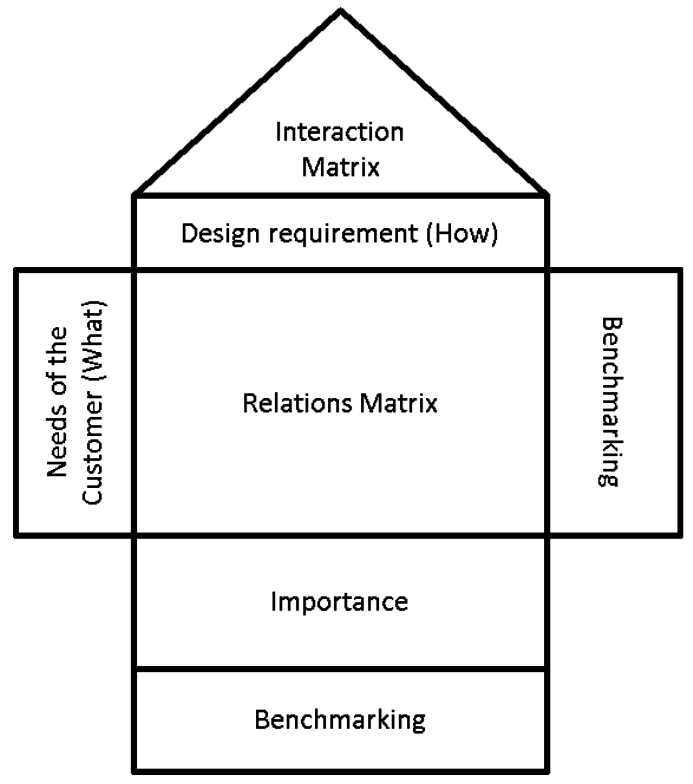
\includegraphics[width=0.7 \linewidth]{HouseOfQuality}
\label{fig:HouseOfQuality}
\caption{House of quality as in the quality function deployment method.}
\end{figure}

\paragraph{House of quality}

\begin{enumerate}
\item Define the \emph{customer needs} (what).
\begin{itemize}
\item e.g. What are actionable results for improving \ldots ?
\item e.g. What is the influence per region to \ldots?
\item What is the cost benefit ratio per region?
\item What is the influence of the marketing budget on \ldots ?
\item e.g. Project has to be completed in $X$ weeks.
\end{itemize}
\item Define the \emph{analytics project requirements} (how).
\begin{itemize}
\item e.g. fast methods which reveal trends vs. detailed analyses
\item e.g. appropriate data (internal or external)
\item e.g. sufficient resources for performing the project
\item e.g. actionable results within time constraint
\item e.g. proper project planning (resources \& time constraint)
\end{itemize}
\item Link them/determine their relationship, i.e. define the \emph{relations matrix}.
\begin{itemize}
\item 0: no relationship, 1: weak, 2: medium, 3: strong
\item e.g. 3 between \textit{questions asking for causes / influences / relations} and \textit{methods and data}
\item e.g. 2--3 between \textit{actionable results} and \textit{appropriate data}, as well as between \textit{actionable results} and \textit{project planning}
\item e.g. 2--3 between all customer requirements and project planning
\item e.g. 2--3 between project completion and project planning
\end{itemize}
\item \emph{Benchmark} the customer needs (what) against the \textit{current status}, \textit{full project} and \textit{parts of the project}.
\begin{itemize}
\item e.g. \textit{current status} generally low but high for project completion
\item e.g. \textit{full project} generally high but low for project completion
\item e.g. \textit{parts of the project} only high for the part(s) it covers and project completion
\end{itemize}
\item Define the \emph{interaction matrix} (interactions of the design requirements (how)).
\begin{itemize}
\item (-- strong negative, - negative, 0 neutral, + positive, ++ strong positive relationship)
\item generally high interactions/correlations, i.e. + to ++
\end{itemize}
\item Determine the \emph{importance} of the design requirements (how).
\begin{itemize}
\item generally high importance, i.e. 60--100\%
\item e.g. 90--100\% of actionable results and project planning
\end{itemize}
\item \emph{Benchmark} the design requirements (how) against the project options.
\begin{itemize}
\item e.g. current status generally low but high for sufficient resources
\item e.g. full project generally high but low for sufficient resources
\item e.g. parts of the project quite similar to current status but a bit more balanced
\end{itemize}
\end{enumerate}

\begin{figure}[H]
\centering
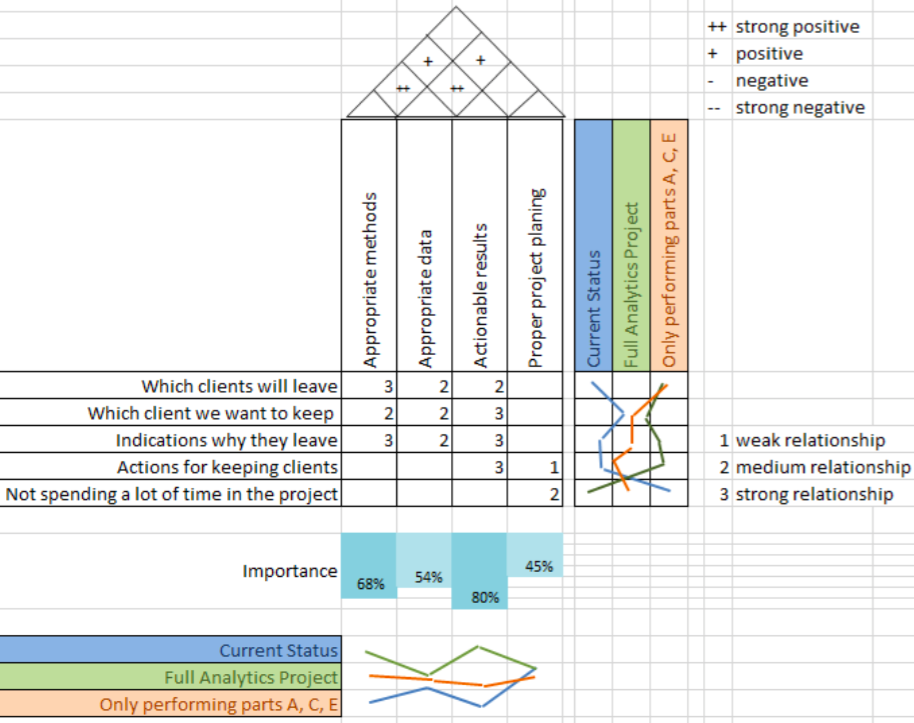
\includegraphics[width=1.05 \linewidth]{HouseOfQualityExample}
\label{fig:HouseOfQuality}
\caption{Example of a house of quality.}
\end{figure}

\paragraph{Requirements}

\begin{itemize}
\item \emph{Expected or basic requirements:} are considered as given and are often unspoken
\item \emph{Normal or performance requirements:} directly mentioned by the customer and which thus can be verbalised
\item \emph{Exciting or emotional requirements:} reflect a need that the client has not appreciated before
\end{itemize}

\begin{figure}[H]
\centering
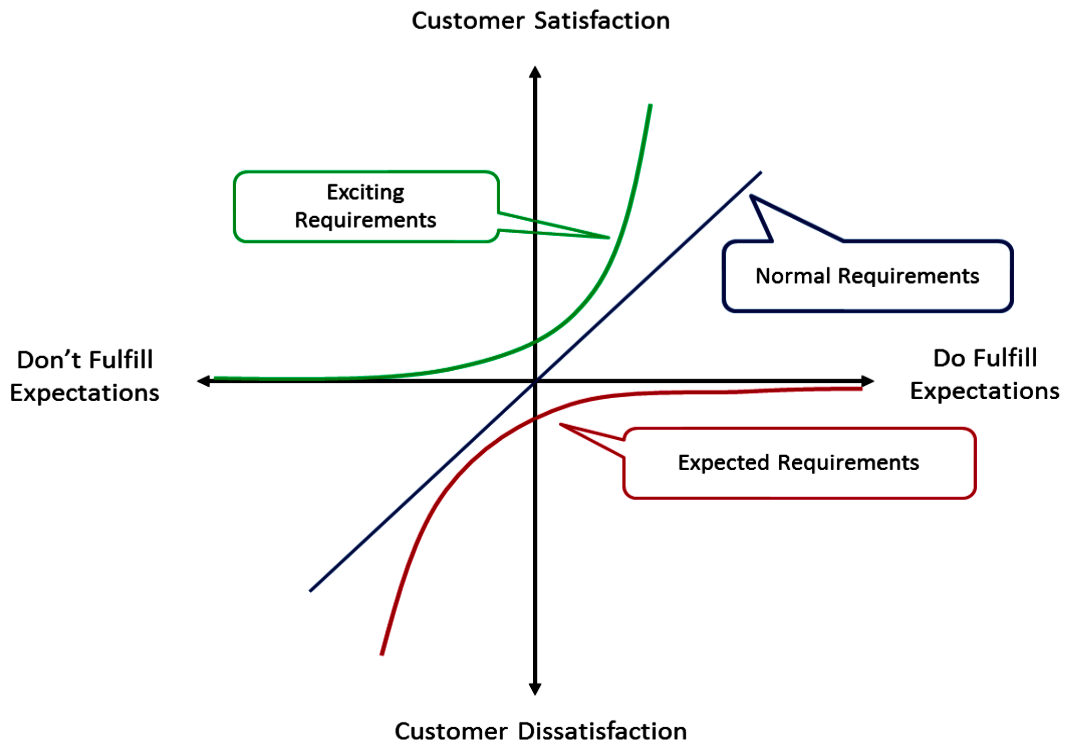
\includegraphics[width=1.0 \linewidth]{CustomerRequirements}
\label{fig:CustomerRequirements}
\caption{Customer requirements as in Kano's model and the quality function deployment model.}
\end{figure}

\paragraph{Conclusion}

\begin{itemize}
\item Very rigorous process that can be applied to any data analytics process
\item Maps the translation or requirements from the business level to the following analytics levels
\item Requires time
\item Recommended for larger projects where a detailed design and process have to be set up in advance with high reliability
\end{itemize}

\subsubsection{Kano's model}

In the Kano model, a \emph{four step approach} is carried out.

\paragraph{Requirements}

\begin{itemize}
\item \emph{Expected requirements} or \emph{must-be requirements} \\
Although not explicitly stated they are taken for granted and constitute basic attributes of each product; if not fulfilled they lead to customer dissatisfaction and if fulfilled they may only lead to non-dissatisfaction
\item \emph{Normal requirements} \\
Connect the customer satisfaction and the level of fulfilment proportionally; they are usually explicitly demanded by the customer
\item \emph{Exciting requirements} or \emph{attractive requirements} \\
These are the differentiating factor; have the greatest influence on customer satisfaction; are usually not explicitly stated nor expected; give additional experience with a product; if not fulfilled there is no dissatisfaction
\end{itemize}

\paragraph{1) Identification of product requirements}

\begin{itemize}
\item What are the associations of the customer when using the product? \\
(e.g. high expectation of immediate actionable results, or expecting just a simple cost analysis)
\item Which problems are associated by the customer with the use of the product? \\
(e.g. tight time schedule, openness to new insights vs. predefined opinions, supporters vs. non-supporters)
\item Which criteria are taken into account when buying the product? \\
(e.g. focus on strategic \& organizational impact (economic buyers), focus on cost, focus on analytical results (technical buyers))
\item Which new features or services would better meet the expectatioins of the customer? Or: What would the customer change in the product? \\
(e.g. quick analyses with actionable outcomes (''quick wins''), just cost analyses, confirmation of existing opinions)
\end{itemize}

\paragraph{2) Construction of the Kano questionnaire}

\begin{itemize}
\item A pair of questions is formulated for each product/service feature: \\
A \emph{functional form} which concerns a reaction if a product has a feature \\
A \emph{dysfunctional form} which conerns a reaction if a product does not have a feature
\item \textit{Possible answers:} \\
I like it that way / It must be that way / I am neutral / I can live with it that way / I dislike it that way
\item \textit{Examples:}
\begin{itemize}
\item \textit{Actionable results:} \\
If we have within two weeks only actionable results which additionally require an increase in the marketing budget in the short run, how do you feel? \\
If we have within two weeks no actionable results which require an increase in the marketing budget in the short run, how do you feel?
\item \textit{Willingness to action on the results:} \\
If you have actionable results from the analysis which require a change of your corporate strategy, how do you feel? \\
If you have no actionable results from the analysis which require a change of your corporate strategy, how do you feel?
\item \textit{Full project vs. parts of the analysis:} \\
If the full data analytics project is performed (with all costs, resources and time), how do you feel? \\
If not the full data analytics project is performed (with all costs, resources and time), how do you feel?
\end{itemize}
\end{itemize}

\paragraph{3) Getting the data from the customers}

\begin{itemize}
\item Standardised questionnaire vs. interview
\item Mail vs. online questionnaire
\item Customer panel vs. randomised potential customer
\end{itemize}

\begin{figure}[H]
\centering
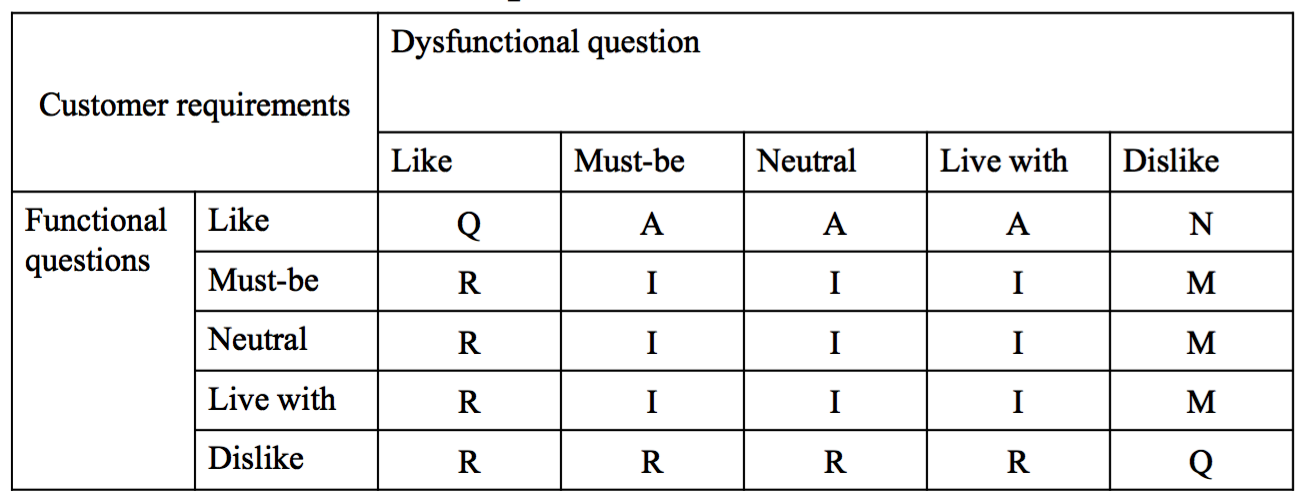
\includegraphics[width=1.05 \linewidth]{KanoScores}
\label{fig:KanoScores}
\caption{Categorization IOT calculate the customer satisfaction index.}
\end{figure}

\paragraph{4) Analyse the results}

\begin{itemize}
\item \emph{Categories:} \\
\emph{A:} attractive, \emph{N:} neutral, \emph{M:} must-be, \emph{R:} reverse, \emph{I:} indifferent, \emph{Q:} questionable
\item Evaluation order: If there is no clearly dominant category: \\
M $>$ N $>$ A $>$ I
\item \emph{Customer satisfaction index:} how strongly a product feature may influence satisfaction or dissatisfaction:
\begin{align*}
\text{Satisfaction} &= \frac{A+N}{A+N+M+I} \\
\text{Dissatisfaction} &= -\frac{N+M}{A+N+M+I}
\end{align*}
\item Plot results as frequencies.
\item The level of \emph{satisfaction} quantifies the impact of \emph{fulfilling} a certain requirement on overall satisfaction.
\item The level of \emph{dissatisfaction} quantifies the impact of \emph{not fulfilling} a certain requirement on overall satisfaction.
\end{itemize}

\begin{figure}[H]
\centering
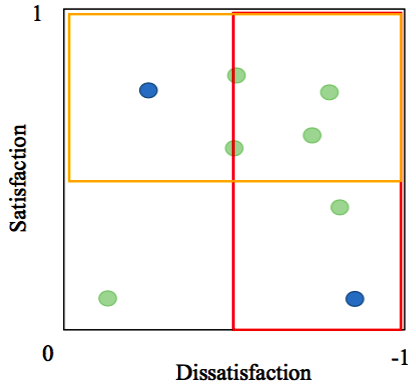
\includegraphics[width=0.5 \linewidth]{KanoFrequencies}
\label{fig:KanoFrequencies}
\caption{Example plot of the correlations between satisfaction and dissatisfaction in the Kano model.}
\end{figure}

\subsection{Set of drivers and relationships to inputs}

\begin{itemize}
\item Main goal: define \emph{inputs} and \emph{outputs}
\item This can be conducted \emph{informally} or \emph{formally} \\
''Formally'' is prefered since it supports communication with the stakeholder.
\item At this stage one is not looking for causual relationships, one is just collecting ideas IOT build up hypotheses (against which the model can later be tested)
\item Determine increasing or decreasing factors (and evaluate their impact on scale).
\item Draw a \emph{Black-box sketch} \\
Make the inputs visible s.t. it can be discussed and challenged, e.g. by technical experts.
\end{itemize}

\subsection{Set of key assumptions related to the problem}

\begin{itemize}
\item In each input/output factor there are \emph{assumptions} implied.
\item These are often \emph{common practice assumptions} which are nowhere explicitly stated.
\item In a project all assumptions have to be listed and assessed.
\end{itemize}

\subsection{Defining key metrics of good performance}

\begin{itemize}
\item The key metric always have to be \emph{measurable}.
\item \textit{Examples:} revenue has to be improved by X\%, no net loss of customers, the production process has to be Y minutes faster per quantity, \ldots
\begin{itemize}
\item \textit{Analysis of a supply chain w.r.t. supply chain risk:} \\
avoidance or reduction of possible business interruption (e.g. to a certain number of days), certain level of manufacturing material available, price stability of manufacturing material
\item \textit{Analysis of insurance claims for fraud cases:} \\
amount of detected fraud cases where the insurance company does not have to pay for claims
\item Reduction of the amount of chemicals in a production process without loss of quality and efficiency: \\
amount of chemical used per quantity compared to a certian threshold, processing time per quantity, number of quantity that does not pass the quality check
\item \textit{Improvement of transport routes of a cargo firm:} \\
reduction in tonne-kilometre while delivering the same or more services/transports, delivering the same tonne-kilometre with less resources
\item \textit{Analysis of non-compliant product sales of a bank:} \\
number of non-compliant product sales found per $X$ customers/per client advisor $Y$
\item \textit{Improvement of the production process of a manufacturing company:} \\
production cost per quantity, production time per quantity, production capacity
\end{itemize}
\end{itemize}

\subsection{Obtaining stakeholder agreement on the approach}

\begin{itemize}
\item This can either be separated from the business problem statement or be integrated.
\end{itemize}

\section{Data}

\paragraph{What has already been done}

\begin{itemize}
\item \textit{Business problem statement:} first assessment of available data, the ''what''
\item \textit{Data analytics problem statement:} the ''how'', set of drivers (i.e. input variables and outcomes), set of relationships between the variables
\end{itemize}

\subsection{Identification and priorization of data}

\paragraph{Identification and priorization}

\begin{enumerate}
\item Decide about the \emph{characteristic} of the input variable (e.g. mean, distribution, text, ect.).
\item Determine \emph{which data can cover this characteristic} (e.g. personal data for determination of the age/distributions of age).
\item Determine which \emph{data types} are most preferable and prioritize them.
\item List all \emph{available data} one already has or one knows they are available.
\item In case of \emph{missing data}, either create an inventory of \emph{additional data} together with the customer or collect it directly.
\item If data are neither available nor collectable in due time, one has to \emph{refine or redefine} the analytical or the busines problem eventually.
\end{enumerate}

\textit{Remarks:}
\begin{itemize}
\item One must become clear about the type of data one needs and one can finally receive/collect.
\item A thorough understanding of the data is paramount.
\end{itemize}

\paragraph{Data definitions}

\begin{itemize}
\item \emph{Population:} includes all the members/items of interest in a study (i.e. the population w.r.t. a data analytics project rarely coincides with the population in the common sense)
\item \emph{Sample:} a subset of the population; is determined randomly and is preferably representative of the whole population
\item \emph{Data set:} (of structured data) is usually an array of data with variables in columns and observations in rows
\item \emph{Variable:} (or field or attribute) is a characteristic of the items of the populaltion
\item \emph{Observation:} (or case or record) is a list of all variable values for a single member/item of a population
\end{itemize}

\subsubsection{Data types}

\paragraph{Hard data vs. soft data}

\begin{itemize}
\item \emph{Hard data:} is collected by scientific observation and measurement (e.g. experiments)
\item \emph{Soft data:}  is explored from inverviews and reflects subjective opinions and preferences
\item \textit{Translation from soft data into hard data:} develop a set of rules to achieve the same behaviour \\
(e.g. operating room optimization: from inverviews with surgeons and management to a computer simulation)
\end{itemize}

\paragraph{Numerical vs. categorical data}

\begin{itemize}
\item \emph{Numerical data:} meaningful arithmetical operations can be performed \\
(e.g. it is possible to compute the mean and standard deviation) \\
\emph{Discrete vs. continuous data:}
\begin{itemize}
\item \emph{Discrete data:} results from a count (e.g. number of customers buying a certain product)
\item \emph{Continuous data:} results from an essentially continuous measurement (e.g. the waiting time of a patient)
\item \emph{Binned data:} was categorized into discrete categories, i.e. bins
\end{itemize}
\item \emph{Categorical data:} otherwise \\
\emph{Ordinal vs. nominal data:}
\begin{itemize}
\item \emph{Ordinal data:}  there is a natural ordering of its possible categories
\item \emph{Nominal data:} otherwise (i.e. there is no such ordering)
\end{itemize}
\end{itemize}

\paragraph{Cross-sectional data vs. time series}

\begin{itemize}
\item \emph{Cross-sectional data:} on a cross-section of a population at a distinct point in time, i.e. without any time-dependeny
\item \emph{Time series:} collected over time (e.g. stock quotes)
\end{itemize}

\paragraph{Structured vs. unstructured data}

\begin{itemize}
\item \emph{Structured data:} can be put into rows and columns
\item \emph{Unstructured data:} otherwise (e.g. a text or a movie)
\item However, data analytics can only be applied to structured data (since its algorithms cannot directly access unstructured data). Thus, unstructured data first has to be structured IOT make it an input for a data analytics process. \\
(e.g. text mining, big data (hadoop, map-reduce), matching fingerprints)
\end{itemize}

\paragraph{Primary vs. secondary data}

\begin{itemize}
\item \emph{Primary data:} is not yet available and has to be measured and collected first \\
(e.g. new reporting data (due to new production processes), new regulatory data (e.g. on how to quantify expected credit losses on financial instruments))
\item \emph{Secondary data:} has already been collected by someone else \\
(e.g. internet, accounting, statistical data (e.g. census), log data in IT systems)
\begin{itemize}
\item Advantage of secondary data: safes time as data is already available; some data is already structured and cleaned
\item Disadvantage of secondary data: may be outdated; may already be processed (or manipulated)
\end{itemize}
\end{itemize}

\paragraph{Meta data}

\begin{itemize}
\item Data about the data, i.e. describes the data
\item (e.g. data when data was collected, purpose of the collection, how the data was collected, size/volume of the data, image resolution, dates of changes in the data, dates of access to the data, tags in social media)
\end{itemize}

\paragraph{Dummy variable}

\begin{itemize}
\item A 0-1 coded variable for a specific category.
\item 1 labels the observations in this category and 0 labels all other observations not in that category.
\end{itemize}

\paragraph{Examples}

\begin{itemize}
\item \textit{book prices on amazon:} hard, numerical, discrete, time series, structured, primary, meta
\item \textit{multiple choice questionnaire:} soft, categorical, ordinal/nominal, cross-sectional, structured, primary, meta
\item \textit{Twitter tweets:} soft, categorical, nominal, cross-sectional/time series, unstructured, primary, meta
\item the following examples may comprise almost all types of data: claims \& customer data of an insurcance company, clinical tests, web page access
\end{itemize}

\subsection{How to collect and get data}

\paragraph{Decision to collect data}

\begin{itemize}
\item One has to identify which kind of data collection will have the most favourable impact on the quality of the actions and recommendations supported by data analytics. \\
This is typically done by a \emph{decision tree}.
\item Without data gathering, a change will be made if:
\begin{align*}
p U + (1-p) = p(U-L) + L > u
\end{align*}
where:
\begin{description}[style=multiline,leftmargin=0.4cm,font=\textbf]
\item[$p$] probability of getting a good outcome, if a change is made
\item[$U$] value (utility) of making a change with good outcome
\item[$L$] value (utility) of making a change with bad outcome
\item[$u$] value (utility) of continuing with the present course
\end{description}
\item But: one can gather data and make decisions based thereon.
\item While the value of information is nonnegative, gathering data also incurs cost.
\item Data will be gathered if:
\begin{align*}
d(q u^\ast + (1-q)u) > u
\end{align*}
where:
\begin{description}[style=multiline,leftmargin=0.4cm,font=\textbf]
\item[$p^\ast$] probability of getting a good outcome, if getting favourable information
\item[$p^{\ast \ast}$] probability of getting a good outcome, if getting unfavourable information
\item[$p$] probability of getting a good outcome, if a change is made \\
$p = qp^\ast + (1-q)p^{\ast \ast}$
\item[$q$] probability of getting favourable information
\item[$u^\ast$] value (utility) of implementing a change, given getting favourable information: \\
$u^\ast = p^\ast (U-L) + L$
\item[$u$] value (utility) of continuing the present course, given getting unfavourable information
\item[$d$] factor by which cost decrease utility
\end{description}
\item $u^\ast$ depends on how much $p^\ast$ differs from $p$. Thus, the degree of change of $p$ with the new information dpends on:
\begin{itemize}
\item the confidence we have in the original value $p$
\item the impact of the data
\end{itemize}
\item Finally, the decision to collect data and which data is very \emph{subjective}, is biased on our \emph{beliefs} and depends on how confident we are in the original probability $p$.
\end{itemize}

\subsubsection{Data collection}

\paragraph{Overview: Data collection}

\begin{enumerate}
\item \emph{Sample design:} determine how to identify the subjects/items
\item \emph{Sample plan:} determine how many subjects/items to identify
\item Determine the \emph{questions} to be asked
\item \emph{Granularity of the experiment:} determine the possible answers to the questions
\item Determine the \emph{control group}
\end{enumerate}

\paragraph{1. Sample design}

\begin{itemize}
\item \emph{(Simple) random sampling}
\begin{itemize}
\item To each subject/item the same chance is allocated to be selected for the sample.
\item Advantage: unbiasedness
\item Disadvantage: if events/subjects/items are very unlikely, it is also very unlikely to have them in a (simple) random sample
\item Thus, it may be advantageous to bias the sampling towards those subject that are of interest. \\
Nevertheless, the analysis has to take into account this bias and the formulas have to be corrected for this bias.
\end{itemize}
\item \emph{Stratified random sampling}
\begin{itemize}
\item divide population into homogenous subpopulations (strata)
\item strata have to be mutually exclusive (i.e. as partitions)
\item to each stratum sampling is applied
\item correction for bias has to be implemented
\item e.g. testing the correctness of Swiss DRG cost code allocations (health care)
\end{itemize}
\item \emph{Full factorial design:} gives the possibility to identify the impact of each factor as well as of possible interactions between the factors in an efficient manner \\
(e.g. regression analysis, ANOVA)
\end{itemize}

\paragraph{2. Sampling plan}

\begin{itemize}
\item \emph{Depends on:}
\begin{itemize}
\item Amount of uncertainty
\item How much does this uncertainty need to be reduced?
\item Degree of error contained in the responses of a subject/item
\end{itemize}
\item \emph{Candidates:} width of the confidence interval, confidence level, power of a test
\item Usual \emph{assumptions:}
\begin{itemize}
\item \textit{Independence:} often given in practice \\
e.g. buying decisions of customers, car accidents
\item \textit{Identically distributed:} often not given in practice \\
Thus, homogenous subclasses are needed for the analysis, but then the sample might be too small for performing meaningful data analytics
\item \textit{No systematic error:} very difficult to detect in practice \\
e.g. drifts or if the subsample is very small
\end{itemize}
\end{itemize}

\paragraph{3. Determination of the questions to be asked / 4. Granulatiry of the experiment}

\begin{itemize}
\item \emph{Primary data:} interview questions and questionnaires
\begin{itemize}
\item \textit{Categorical:} \\
Format: $\lbrace$black, silver, red, white, \ldots$\rbrace$, $\lbrace$yes, no$\rbrace$, $\lbrace$fully agree, partially agree, \ldots$\rbrace$ \\
e.g. preferred characteristics of a new product (such as preferred colour) \\
e.g. to find out how many foreign languages people are speaking \\
e.g. to find out what people think about the political agenda of a party
\item \textit{Semantic differential:} \\
Format: user friendly vs. cumbersome, slow vs. fast, confusing vs. clear \\
e.g. to determine personality traits
\item \textit{Rank-order:} \\
e.g. to rank the most important benefits of a product \\
e.g. to find out the five most important benefits of a new product \\
e.g. to find out the most and least useful feature of a new product
\item \textit{Multiple choice:} \\
e.g. to test analytical thinking of job candidates
\end{itemize}
\item \emph{Secondary data}
\begin{itemize}
\item Since secondary data is already available, one has to find and assess it for appropriateness.
\item Questions to be asked: \\
kind of data, data inventories, source of data, primary purpose for collecting the data, who collected the data, when was it collected, raw data vs. cleaned data, meta data, coverage of the data, aggregate basis vs. single basis, type of data, volume, who is responsible for the data, who has access to the data, can the data be downloaded/is it accessible in due time, is there a description of the recorded data fields, from how many systems/sources is the data, cost for accessing the data, who are the users of the data, are there reports using the data, are there identifiers that facilitate merging data, who has the rights to change data afterwards, is there a delay in recording and/or transferring data?
\end{itemize}
\end{itemize}

\paragraph{5. Determination of the control group}

\begin{itemize}
\item To compare the test results with the current or standard status, a control group is chosen out of the same population.
\item e.g. as in clinical studies or in marketing
\end{itemize}

\subsection{Harmonizing, rescaling and cleansing of data}

\paragraph{Reasons for data cleaning}

\begin{itemize}
\item \emph{Secondary data (pre-existing databases):} data is collected for other purposes, i.e. quality of data is driven by what was originally important, and thus there is so far no need to satisfy the quality requirements for the new analysis
\item \emph{Primary data (data collected via surveys):} individuals may get fatigued when filling out an extensive survey and thus may simply put default values (usually neutral or extremely positive or negative); false answers if individuals got offended by questions; most people simply refuse to fill out a survey
\end{itemize}

\paragraph{Process of data cleaning}

\begin{enumerate}
\item \emph{Raw Data}
\item \emph{Technically correct data}
\begin{itemize}
\item each value can be recognized belonging to a certain variable
\item each value is stored in a data type that represents the value domain of the real-world
\end{itemize}
\item \emph{Consistent data}
\begin{itemize}
\item missing values, special values, (obvious) errors and outliers are either removed, corrected or imputed
\item data is consistent with constraints based on real-world knowledge about the subject
\item i.e. data is fit for the analysis
\end{itemize}
\end{enumerate}

\paragraph{Common issues in data cleaning}

\begin{itemize}
\item Assess \emph{technical correctness}
\begin{itemize}
\item range of valid responses
\item invalid data responses (e.g. letters in number fields)
\end{itemize}
\item Assess \emph{consistency}
\begin{itemize}
\item inconsistent data encodings (e.g. different abbreviations for countries)
\item suspicious/questionable data responses (do the outliers make sense?)
\item suspicious distribution of values (use descriptive statistics to identify, e.g. histogramms, box plot, etc.)
\item suspicious relationships between fields (identify correlations, e.g. factor analysis, etc.)
\end{itemize}
\item Handling \emph{null or missing values}
\begin{itemize}
\item Deletion: always drop
\item Deletion when necessary: only drop observation unless required for analysis
\item Imputing a value: use of regression to predict an answer (but this might understate the uncertainty)
\item Randomly imputing a value: rerun analysis for all possible outcomes and weight by regression-based probability
\end{itemize}
\end{itemize}

\paragraph{Issues when combining data from different sources}

\begin{itemize}
\item The \emph{level of granularity} may be different. \\
\textit{Solution:} either skip inconsistent variables unless needed or apply methods for missing values
\item The \emph{data architecture} may be different (e.g. NA, na, space, etc.) \\
\textit{Solution:} harmonize before aggregating the data
\item Data may be \emph{stored in different ways} (e.g. in several databases with different structure). \\
\textit{Solution:} define a record which has enough fields to contain the information of each of the databases
\item There may be \emph{different weights} of the observations (e.g. based on 10,000 vs. 100 responses). \\
\textit{Solution:} introduce a weighting field
\end{itemize}

\paragraph{Helpful tips and tricks for data cleaning}

\begin{itemize}
\item create a \emph{date stamp}
\item create a field identifying the \emph{source}
\item create new fields with \emph{computed values} (i.e. if information is required that is not yet in the database)
\item delete fields that have the same value accross all datasets
\item store input data for each stage (i.e. raw, technically correct, consistent, aggregated, formatted)
\end{itemize}

\paragraph{Final checks on data quality}

\begin{itemize}
\item \emph{the 10 C's}
\begin{itemize}
\item \emph{Completeness}
\item \emph{Correctness}
\item \emph{Currency:} is the data obsolete?
\item \emph{Collaborative:} is the data based on one opinion or on a consensus of experts?
\item \emph{Confidential:} is the data secure from unauthorized use?
\item \emph{Clarity:} is the data legible and comprehensible?
\item \emph{Common format:} is the data in a format easily to be used?
\item \emph{Convenient:} convenient and quick access to data?
\item \emph{Cost-effective}
\end{itemize}
\item \emph{ACCURATE}
\begin{itemize}
\item \emph{Accurate:} fair and free from bias? arithmetical or grammatical errors?
\item \emph{Complete}
\item \emph{Cost-beneficial}
\item \emph{User-targeted:} style, format, detail and complexity address the the nedds of the users?
\item \emph{Relevant:} communicated to the right person?
\item \emph{Authoritative:} reliable source?
\item \emph{Timely:} does the receiver of the information have enough time to decide appropriate actions?
\item \emph{Easy to use:} understandable to users?
\end{itemize}
\end{itemize}

\subsection{Discovery of relationship in data}

\paragraph{Overview}

\begin{itemize}
\item \emph{Describe:} How do I develop an understanding of the content of my data?
\begin{itemize}
\item \emph{Processing:} How do I clean and separate my data?
\begin{itemize}
\item Filtering
\item Imputation
\item Dimensionality reduction
\item Normalization and transformation
\item Feature Extraction
\end{itemize}
\item Aggregation
\item Enrichment
\end{itemize}
\item \emph{Discover:} What are the key relationships in the data?
\begin{itemize}
\item Clustering
\item Regression
\end{itemize}
\end{itemize}

\paragraph{Discovery of relationship in data}

\begin{itemize}
\item \emph{Filtering:} identify data based on its absolute or relative values
\begin{itemize}
\item use \textit{relational algebra projection and selection} IOT add or remove data based on its value
\item use \textit{outlier removal, exponential smooting} and either \textit{Gaussian or median filters}
\end{itemize}
\item \emph{Imputation:} fill in missing values in data
\begin{itemize}
\item generate values for missing data using \textit{random sampling} or \textit{Monte Carlo Markov Chain methods}
\item use \textit{mean, regression models} or \textit{statistical distributions} based on existing observations
\end{itemize}
\item \emph{Dimensionality reduction:}
\begin{itemize}
\item determine correlation accross different dimensions using \textit{principle component analysis} or \textit{factor analysis}
\item in unstructured text data: use \textit{term frequency/inverse document frequency} IOT identify the importance of a word \\
(use the inverse frequency since the important terms usually have a low frequency)
\item create a fixed number of features which form the indices of an array using \textit{feature hashing}
\item use \textit{sensitivity analysis} and \textit{wrapper methods} when important features are not known
\item use \textit{self-organizing maps} and \textit{Bayes nets} IOT understand the probability distribution of data
\end{itemize}
\item \emph{Normalization and transformation:} reconcile duplication representations
\begin{itemize}
\item correct duplicate data elements with \textit{de-duplication}
\item \textit{normalization} ensures your data stays within a common range
\item \textit{format conversion} is typically used when data is in binary format
\item for frequency data: use \textit{fast Fourier transforms (FFT)} and \textit{discrete wavelet transforms}
\item for geometric data defined over Euclidean: use \textit{coordinate transformations}
\end{itemize}
\item \emph{Feature Extraction:} determine the set of features with the highest information value to the model
\begin{itemize}
\item features can be filtered out and tested with statistics, which is independent of the finally applied model
\item with \textit{wrapper methods} (e.g. regression, k-nearest neighbour), one evaluates feature sets by constructing models and measuring performance
\end{itemize}
\item \emph{Aggregation:} collect and summarize the data
\begin{itemize}
\item use \textit{basic statistics} (raw counts, means, medians, standard deviations, ranges) IOT summarize data
\item use \textit{box plots} and \textit{scatter plots} IOT provide compact representation
\item use \textit{''baseball card'' aggregation} IOT summarize all the information available on an entity
\end{itemize}
\item \emph{Enrichment:} add new information to the data
\begin{itemize}
\item use \textit{annotation} IOT track source information and other user-defined parameters (e.g. which ZIP code belongs to which canton)
\item use \textit{relational algebra rename and feature addition} (e.g. geography, weather) IOT process certain data fields together or use one field to compute the value of another
\end{itemize}
\item \emph{Clustering:} segment the data to find natural groupings
\begin{itemize}
\item \textit{connectivity-based} methods: hierarchical clustering
\item \textit{centroid-based} methods: use \textit{k-means} when the number of clusters is known, use \textit{x-means} or \textit{Canopy clustering} when the number is unknown
\item \textit{distribution-based} methods: \textit{Gaussian mixture models}
\item \textit{density-based} methods: \textit{fractal and DB scan} are useful for non-elliptical clusters
\item \textit{graph-based} methods: useful when you only have knowledge of how one item is connected to another
\item \textit{topic modeling:} for segmentation of text data
\end{itemize}
\item \emph{Regression:} determine which variables are important
\begin{itemize}
\item \textit{tree-based methods:} when structure of data is unknown
\item \textit{generalized linear models:} when statistical measure of importance is needed
\item \textit{regression with shrinkage} (e.g. LASSO, elastic net) and \textit{stepwise regression} when statistical measure of importance is not needed
\end{itemize}
\end{itemize}

\subsection{Documentation and reporting of findings}

\begin{itemize}
\item Raw data and relationships will not attract attention of your stakeholders.
\item Tie your findings to the analytics problem and from there to the business problem.
\item State the impact of your findings to the business and complement this with recommendations.
\item Document exceptional or more pronounced relationships.
\item Document as well the data warehouses IOT make them usable for external parties (there might be requests to revisit the data months or years after the analysis is done).
\end{itemize}

\subsection{Re-definition of the business and analytics problem statement by use of the data analytics result}

\emph{Solid data and relationships} will allow you to find that:
\begin{itemize}
\item the \textit{true constraints of the system} are not as originally assumed and thus the analytics problem needs to be \emph{reframed}. Also, maybe only a part of the original question can be answered.
\item the business problem itself missed a key facet (e.g. unexpected relationship, time-series effect, etc.) that needs to be \emph{included}.
\end{itemize}

\section{Identification of problem solving approaches and appropriate tools}

\begin{figure}[H]
\centering
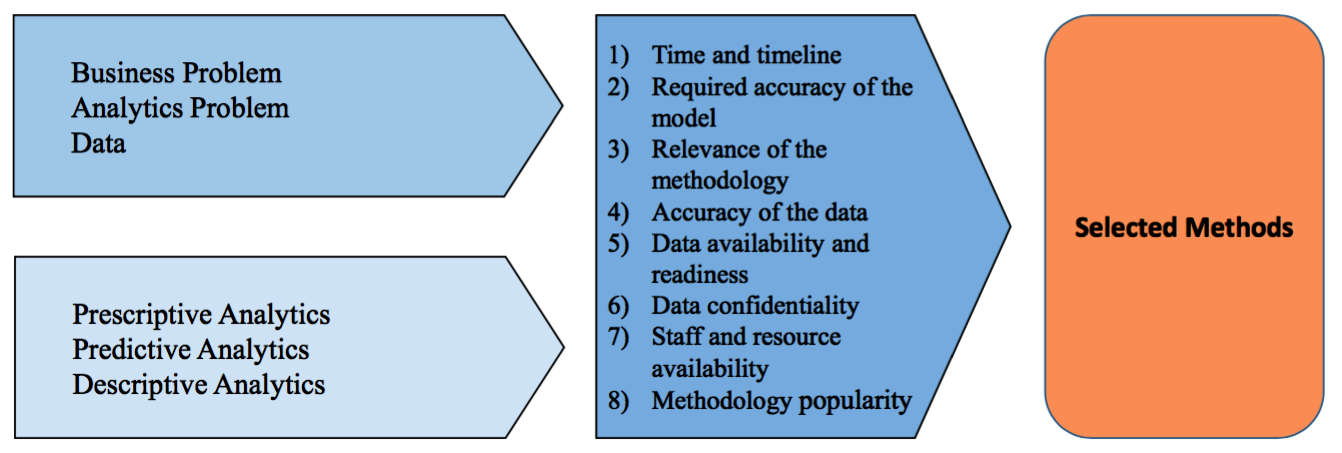
\includegraphics[width=1.0 \linewidth]{ProblemSolvingApproachesMethods}
\label{fig:ProblemSolvingApproachesMethods}
\caption{Process of selecting methods.}
\end{figure}

\subsection{Identify available problem solving approaches/methods}

\begin{enumerate}
\item \emph{Time and timeline}
\begin{itemize}
\item typically tight deadlines
\item thus often no time for experiments or testing new methods
\item consequently, fast and familiar methods are preferred
\end{itemize}
\item \emph{Required accuracy of the model}
\begin{itemize}
\item accuracy of the results depends on the aggregation/granularity of the model and the quality and readiness of the data
\item thus, if quality and accuracy of data is poor, sophisticated models do not provide any additional value
\end{itemize}
\item \emph{Relevance of the methodology}
\begin{itemize}
\item the business problem statement and the analytics problem framing often point the direction to a methodology
\item thus it is important to understand the goal of the analytics project (e.g. is it descriptive, predictive or prescriptive)
\item also, one has to adapt the methodology (or maybe even the goal) to the data analytics awareness of the stakeholder
\end{itemize}
\item \emph{Accuracy of the data}
\begin{itemize}
\item accuracy of the data restricts the pool of possible methods
\item e.g. granular time series models vs. simple regression analysis
\end{itemize}
\item \emph{Data availability and readiness}
\begin{itemize}
\item data might be available but might not be readily accessible, might only be available in very poor quality, or the quality and relevance of the data might not be known at all
\item e.g. data about standard products vs. special products
\item e.g. data stored on old IT infrastructure
\end{itemize}
\item \emph{Data confidentiality}
\begin{itemize}
\item classification of data might be internally regulated or by data protection laws
\item thus, data might be available only highly anonymized and/or aggregated
\item e.g. patient data from hospitals
\end{itemize}
\item \emph{Staff and resource availability}
\begin{itemize}
\item there are differend experts for different areas, e.g. experts on statistics, operations research, pricing, ect.
\item lack of experts can often delay a project for several weeks
\item there might also be restrictions due to limited available licenses of analytics software (especially if one has to work on the premises of the customer)
\end{itemize}
\item \emph{Methodology popularity}
\begin{itemize}
\item sometimes the customer asks for a certain method to be applied
\item however, it is in the responsibility of the data analytics professional to apply the most accurate/adequate methods but not only the most popular
\end{itemize}
\end{enumerate}

\subsection{Descriptive methods}

\paragraph{Examples}

\begin{itemize}
\item mean, median, mode, variance, standard deviation
\item scatterplot, histogram, boxplot, steam-leaf plot
\end{itemize}

\paragraph{When to use descriptive methods?}

\begin{itemize}
\item for reducing, summarizing and grouping data
\item there is no dependent variable, i.e. the aim is to only describe what the data shows
\item to simplify large amounts of data
\item if one is unfamiliar with the data set and thus a feeling for the data first needs to be build up
\end{itemize}

\subsection{Predictive methods}

\begin{itemize}
\item \emph{Regression:} techniques for estimating relationships among variables and building up an understanding of which variables are important in predicting future values
\begin{itemize}
\item consists of a dependent variable (to be estimated) and of independent variables (predictors)
\item \emph{Linear regression}
\item \emph{Step-wise regression:} inclusion or deletion of the independent variable step by step based on some statistical measure (e.g. t-test or F-test); \textit{forward selection} (starting with no independent variable and adding then the variable which improves the model most by its inclusion) vs. \textit{backward selection} (start with all variables included and deleting then the variable which improves the model most by its deletion)
\item \emph{Shrinkage regression} (e.g. Ridge regression or Lasso): if there are more variables than observations, least-square estimators do not exist; a \textit{penalty} (additional constrations on the coefficients) can overcome the issue of $(X^T X)^{-1}$ being singular
\item \emph{Logistic regression:} the regression case where the dependent variable is categorical, especially \textit{binary}; important in credit scoring models and generally in the financial risk modelling area \\
e.g. also to determine which customers will respond to a new marketing campaign
\item Test of performance: $R^2$, $R^2_\text{adj}$ ($R^2_\text{CS}$ or $R^2_\text{McF}$ or likelihood ratio test for logistic regression), AIC, BIC, accuracy/error rate, ROC
\end{itemize}
\item \emph{Clustering:} techniques for the segmentation of data into naturally similar groups
\begin{itemize}
\item \emph{Hierarchical clustering:} for an ordered set of clusters with observation precision
\item \emph{k-means clustering:} to partition $n$ observations into $k$ clusters, where $k$ is known (e.g. centroid base method, where one aims to minimize the distance (as sum of the squares) of each point in the cluster to the cluster centre)
\item \emph{x-means clustering:} if the number of clusters $x$ is unknown
\item Test of performance: ROC, sum of squared error (SSE), measures the compactness of a cluster or comparison with a given cluster structure (rand index)
\end{itemize}
\item \emph{Classification:} techniques for the prediction of the group membership of the observations
\begin{itemize}
\item \emph{Decision trees:} the algorithms start at the top and at each node a variable is chosen/determined that splits best the sample of observations; typically used when a transparent model is needed; e.g. CART, MARS, random forest, bagging
\item \emph{k-nearest neighbours:} non-parametric alogrithm that classifies a point under consideration of the $k$-nearest neighbours to this point; typically used when the data dimension is not too high
\item \emph{Neural networks:} the algorithms learn features in the data by changing the weights between the nodes based on learning rules
\item if one does not know where to start: use \emph{Support Vector Machine (SVM)} or \emph{Naïve Bayes}
\item Test of performance: accuracy/error rate, ROC
\end{itemize}
\item \emph{Statistical inference:} drawing conclusions based on data
\begin{itemize}
\item e.g. confidence intervals, hypotheses testing, analysis of variance (ANOVA)
\item \emph{Design of experiments:} planning, conducting, analyzing and interpreting control test; it aims to quantify the effects of values of the output parameters by controlled variation of the input factors
\end{itemize}
\item \emph{Simulation:} the design of a model of a real-world system or process, executing the model and analyzing the output of the model; the intention is learning by doing
\begin{itemize}
\item Test of performance: analysis of the difference between the model and the status quo.
\end{itemize}
\end{itemize}

\subsection{Prescriptive methods}

\begin{itemize}
\item \emph{Mathematical optimisation}
\begin{itemize}
\item generall mathematical optimization problem: minimize $f(z)$ (objective function), subject to $f_i(x) \leq b_i$ (constraint functions)
\item \emph{Linear programming:} optimum in a linear mathematical model subject to linear constraints
\item \emph{Integer programming:} special case of linear programming where variables take integer values only
\item \emph{Nonlinear programming:} either the objective function or the constraints are non-linear
\item \emph{Metaheuristics:} uses intensification and diversification
\item also: calculus of variations, e.g. Euler-Lagrange equations, the generalization of the optimal control theory, dynamic programming (derives overall solution from solutions of the sub-problems)
\end{itemize}
\item \emph{Stochastic optimisation}
\begin{itemize}
\item Generally: minimize the loss function $L = L(\theta)$ where $\theta$ is the $n$-dimensional vector of parameters that are being adjusted
\item but: either there is a random noise in the measurement, i.e. $y(\theta) = L(\theta) + \epsilon(\theta)$ and/or there is a random choice made in the search direction of the iteration algorithm
\item measurement with noise: \emph{stochastic approximation} that is a recursive update rule (e.g. Robbins-Monro algorithm)
\item random search: \emph{simulated annealing}
\end{itemize}
\item \emph{Simulation}
\begin{itemize}
\item \emph{Discrete event simulation} (e.g. patients running through the operating room process)
\item \emph{Markov models} or \emph{queuing models:} analyze queues where the queue lenghts and the waiting time can be determined (e.g. production processes)
\item \emph{Agent-based modelling (ABM):} simulates the actions and interactions of autonomous agents which are assigned with rules (e.g. product launch in the market where the behaviour of the customers and the competitors are simulated)
\item \emph{Monte Carlo simulation:} based on generated random samples which follow (parametric or non-parametric) statistical distributions and interdependencies (e.g. financial risk models or the development of required capital or equity)
\item \emph{System dynamics:} understand the interactions over time in a complex dynamic system; often implying feedback and reinforcing loops (e.g. simulation of a location strategy of a country)
\item General examples: optimisation of a production line in a plant of a manufacturing company
\end{itemize}
\end{itemize}

\subsection{Selection of software tools}

\paragraph{Dimensions of software}

statistical capabilities, data mining, simulation, optimization, visualization/reporting, user-friendliness, costs, maintenance, transparency, \ldots

\paragraph{Available software}

\begin{itemize}
\item \emph{Microsoft Excel:} regression; all companies have it, VBA, add-ons like $@$Risk
\item \emph{R:} statistical computing and graphics, regression, clustering, classification; scientific standard, open source, many packages
\item \emph{Python:} high-level programming language, e.g. clustering; open source \\
\emph{Pandas:} high-performance, easy-to-use data structures and data analysis tools for Python, especially to manipulate numerical tables and time series, clustering; open source
\item \emph{MATLAB:} simulations; proprietary
\item \emph{KNIME} (Konstanz Information Miner): data mining, maching learning, reporting/visualization, clustering, classification; R and WEKA integration, Java based, open source
\item \emph{Rapidminer:} machine learning, data/text/web mining, predictive and business analytics; partly free
\item \emph{WEKA:} data preprocessing, regression, clustering, classification, feature/attribute selection, and visualization; open source
\item \emph{SAS:} statistical programming language for data analytics, data management, business intelligence, risk management, supply chain management, regression, classification
\item \emph{IBM SPSS Statistics:} addresses the entire analytical process from planning and data collection to analysis, reporting and development, regression, classificatioin; professional vendor suite, licensing system
\item \emph{SQL:} structured query language; language for managing structure data (i.e. data in a relational database management system); used in all database types like oracle, SAP, IBM DB, Microsoft etc.
\item \emph{Apache Hadoop:} open-source software framework in Java for distributed storage and distributed processing of very large data sets
\item \emph{.NET framework:} developed by Microsoft, e.g. C\#
\item \emph{Java}
\item \emph{Julia:} high-level dynamic programming language used for scientific computing, machine learning, data mining, large-scale linear algebra, distributed and parallel computing; very efficient and effective language
\item \emph{System Dynamics/ABM/discrete events software:} PowerSim, Vensim, AnyLogic
\end{itemize}

\section{How to set up and validate models}

\paragraph{Choosing a good model}

\begin{itemize}
\item Good models depend on all previous steps, i.e. framing the business and analytics problems, acquiring, exploring and cleansing the data, identification of problem solving approaches.
\item The tools should actually be chosen based on the requirements of the approaches and models. \\
In practice, though, tools can also be given which then define which models have to be applied.
\item Typically, there is a class of models that seems most appropriate to model the data. \\
In practice, one chooses several types of models from such a class, fits them to the data, and selects the best.
\end{itemize}

\paragraph{Collaboration of involved people}

\begin{itemize}
\item \emph{Business expert:} should have a clear view of the required characteristics to be modelled \\
(e.g. a practioneer, such as a doctor responsible for the operating room management)
\item \emph{Data owner:} should known how to bring the data with the needed characteristics together and create the required data structure for the data analyst \\
\textit{Remark:} often a lot of data cleansing occurs during the model development since each modelling type has its own data obstacles.
\end{itemize}

\paragraph{Qualities of a model}

After several models are fit, one has to assess their performance and consider how the models will be used later.

\begin{itemize}
\item \emph{Precision:}
\begin{itemize}
\item Regression: $R^2$ has to be as close as possible to 1.
\item Classification: The error rate, i.e. the proportion of incorrectly classified items must be as close as possible to 0.
\end{itemize}
\item \emph{Robustness:}
\begin{itemize}
\item Low sensitivity to random fluctuations, missing data or data that changes over time
\item Little dependencies on the training data
\item e.g. regressions or when developing simulations
\end{itemize}
\item \emph{Concision/parsimony:}
\begin{itemize}
\item Rules (conditions, constraints) of a model should be as simple as possible and there should be as few such rules as possible
\end{itemize}
\item \emph{Explicit results:}
\begin{itemize}
\item Rules of a model should be understandable, accessible and explicit (i.e. easy to implement)
\item Very often of importance (maybe except for simulations)
\end{itemize}
\item \emph{Diversity of types of data processed:}
\begin{itemize}
\item A model should be applicable to the available type of data (e.g. discrete, categorical, time dependent, missing)
\item e.g. when analysing messages on social media platforms
\end{itemize}
\item \emph{Speed of the model development:}
\begin{itemize}
\item Fast application of the model (i.e. (near) real-time)
\item Model's training, testing and adaptions should be processed within a reasonable time.
\item e.g. if model should be used as trading strategy
\end{itemize}
\item \emph{Possibility of parameter setting:}
\begin{itemize}
\item Possibility to influence the parameter setting
\item e.g. in classification, clustering or when developing simulations
\end{itemize}
\end{itemize}

\paragraph{Parameter learning/parametric modelling}

\begin{itemize}
\item \emph{Goodness-of-fit:} shows how well a model is fitting the data \\
\begin{itemize}
\item $R^2$ or $R^2_\text{adj}$ for regression
\item Akaike information criterion (AIC) or Bayes information criterion (BIC) for time series models
\item likelihood ratio test (expansions of a model compared to the simpler base model)
\item $R^2_\text{CS}$ or $R^2_\text{McF}$ or likelihood ratio test for logistic regression
\item linear discriminant analysis (Wilk's lambda)
\item accuracy/error rate, ROC
\item p-value in inference
\end{itemize}
\item \emph{Accuracy} and \emph{error rate:} \\
Accuracy = percentage of correct classifications \\
Error rate = percentatage of incorrect classifications
\item \emph{Generalization vs. overfitting:}
\begin{itemize}
\item \emph{Generalization:} property of a model where the model has a generalized application to data that was not used to build the model \\
I.e. when the model is not adequately complex, it becomes very inaccurate.
\item \emph{Overfitting:} the tendency of data mining procedures to tailor models to the training data, at the expense of generalization to data that are not used to build the model \\
i.e. when the model is too complex and incorporates idiosyncracies of the training set \\
This causes performance to decline.
\begin{figure}[H]
\centering
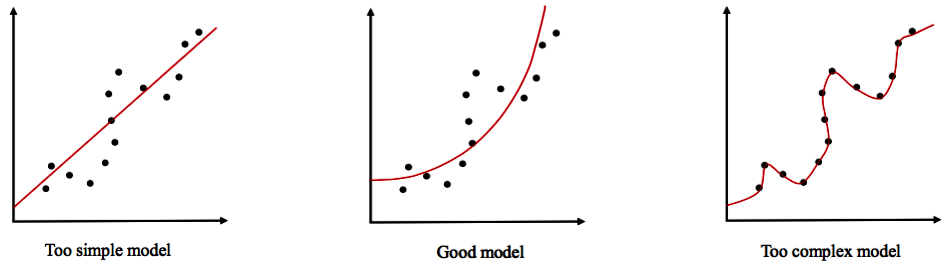
\includegraphics[width=1.05 \linewidth]{GeneralizationVsOverfitting}
\label{fig:GeneralizationVsOverfitting}
\caption{Generalization vs. overfitting.}
\end{figure}
\end{itemize}
\item \emph{Holdout set generalization performance:} the data set (the population) is split into (at least) two subsets.
\begin{itemize}
\item \emph{Training set:} set of data on which the model is fitted and the model parameters are determined
\item \emph{Holdout} or \emph{test set:} used to test the performance of the previously developed model
\item Rule of thumb: app. 70\% of the data are allocated to the training set, while app. 30\% of the data are allocated to the holdout set.
\item Size of the training set: \\
A small training set can easily result in a low error rate in the training phase but will probably results in a high error rate in the testing phase. \\
Contrary, if the training set is too large a model can be less efficient in the training phase but will perform better in the testing phase.
\item Disadvantage: it gives only a single estimate (i.e. a point estimate) of the generalization performance.
\end{itemize}
\item \emph{Cross-validation:}
\begin{itemize}
\item Split the data set into $k$ partitions/folds (usually $k \in \lbrace 5,10 \rbrace$)
\item Cross-validation iterates the training set and holdout set $k$ times, i.e. in each iteration of the cross-validation a different fold is chosen as the holdout set.
\item In each iteration $\frac{k-1}{k}$ of the data is used for training and $\frac{1}{k}$ is used for testing.
\item Based on the performance estimates of all the $k$ folds one can compute the average and standard deviation of the generalization performance. \\
Rule of thumb: the training set should be at least 1,000 items, but for a sufficiently robust model one needs at least 350--500 items.
\end{itemize}
\begin{figure}[H]
\centering
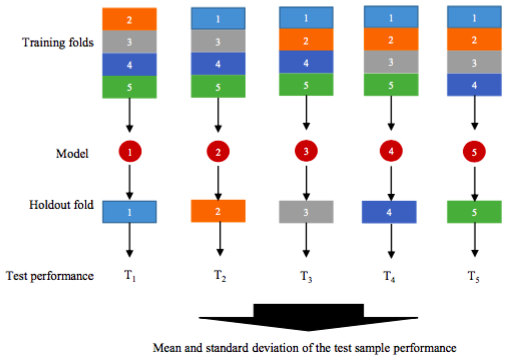
\includegraphics[width=0.9 \linewidth]{kFoldCrossValidation}
\label{fig:kFoldCrossValidation}
\caption{The method of k-fold cross-validation.}
\end{figure}
\end{itemize}

\paragraph{Receiver Operating Characteristic (ROC)/Gini Index}

\begin{itemize}
\item Measures of the \emph{Receiver Operating Characteristic (ROC):}
\begin{itemize}
\item Accuracy $= (\alpha+\delta)/(\alpha+\beta+\gamma+\delta)$
\item True positive rate $=\delta/(\gamma+\delta)$ \\
(sensitivity)
\item True negative rate $=\alpha/(\alpha+\beta)$ \\
(specificity)
\item False positive rate $=\beta/(\alpha+\beta)$ \\
(1-specificity)
\item False negative rate $=\gamma/(\gamma+\delta)$ \\
(1-sensitivity)
\end{itemize}
\begin{figure}[H]
\centering
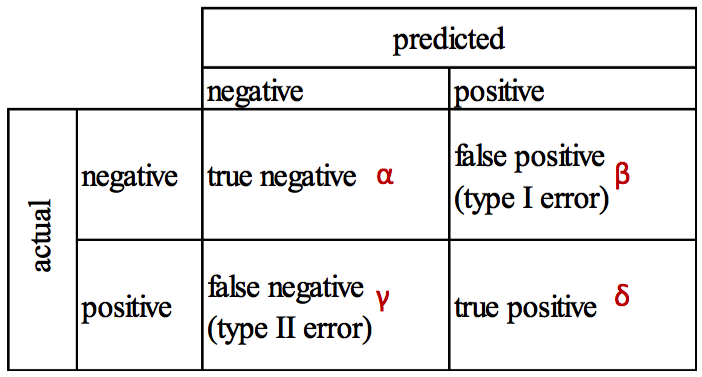
\includegraphics[width=0.8 \linewidth]{ROCTable}
\label{fig:ROCTable}
\caption{Error types of the ROC.}
\end{figure}
\item \emph{Gini index:}
\begin{align*}
\text{Gini-index} &= \frac{A}{A+B}
\end{align*}
The Gini index is in the range of $[0,1]$. The closer the Gini index to 1, the closer is the stastical model to the perfect model.
\begin{figure}[H]
\centering
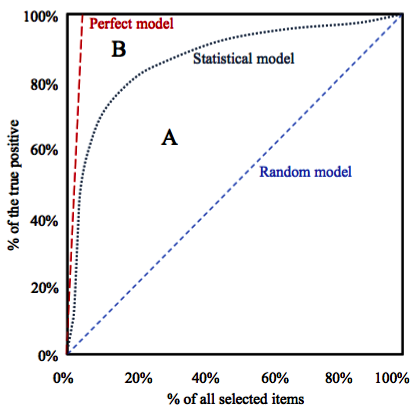
\includegraphics[width=0.7 \linewidth]{ROCCurve}
\label{fig:ROCCurve}
\caption{ROC curves of differen statistical models IOT compute the Gini index.}
\end{figure}
\end{itemize}

\section{The deployment of a model}

\paragraph{Model deployment}

Deployment is the implementation of the data analytics model into an IT or computer system for its use on a regular basis.

\paragraph{Implementation in IT systems}

IOT elaborate the implementation plan:
\begin{itemize}
\item What is the concept of operations (CONOP) of the current system/process? \\
(feedback and acceptance of end users? a solution should interact with the current system that is maximally helpful but minimally disruptive)
\item What is the legacy/computing/processing/operational environment? \\
(familiarize yourself with the system's configuration management system and any leftover software, hardware and methods)
\item What are the available interface mechanisms/processes? \\
(existing application program interface as part of the system specification; ask for documentation; coordinate with system developer IOT avoid conflict)
\item At what point in the processing stream can data be injected? \\
(when is it possible to read/write/update data in the system architecture; synchronize with actions)
\item What are the political/organizational considerations for interaction with the systems? \\
(clearly understand organizational policies regarding the system)
\end{itemize}

\textit{Further remarks:}
\begin{itemize}
\item The four most common ways of deploying models in data mining are:
\begin{itemize}
\item Data mining tool or cloud (app. 45\%)
\item Programming language, e.g. Java, C, VB (app. 15\%)
\item Database and SQL script (app. 25\%)
\item PMML: Predictive model and mark up language (app. 15\%)
\end{itemize}
\item Before requesting data and developing a model, make sure that the data will continue to be captured in the future.
\item Failing in the implementation phase means failing in the project.
\end{itemize}

\paragraph{Availability for users}

Make the model available to the users and train the users.

The model will only be available for users after:
\begin{itemize}
\item model was tested in production for several months with volunteers, in parallel to the previous tool.
\item champion-challenger strategies are implemented and evidently yield better results.
\item a proper take-over phase and training.
\end{itemize}

\textit{Further remarks:}
\begin{itemize}
\item The specification of the model should not be revealed to the end users (otherwise the model might not anymore serve its purpose).
\item Users need to be well trained and understand the background of the models and tools.
\item Training involves: objectives of the model, principles of the tool, limitations, methods for using the tool, contributions of the tool, operational and organizational consequences
\end{itemize}

\paragraph{Monitoring and maintenance}

\begin{itemize}
\item \emph{Monitoring and maintenance plan:}
\begin{itemize}
\item which results may require updating and why
\item how will updating be triggered (regular updates, trigger event, performance monitoring)
\item how will updating be performed
\item summary of the results of the updating process
\end{itemize}
\item \emph{Types of monitoring:}
\begin{itemize}
\item \textit{One-off monitoring:} whenever a new data mining application is put in use
\item \textit{Ongoing monitoring:} \\
\textit{Population stability:} understand how the target population changes over time \\
\textit{Scorecard performance:} understand the benefits of having the right information available when making decisions \\
\textit{Decision management:} understand how the model degradation may affect the quality of the portfolio
\end{itemize}
\end{itemize}

\paragraph{Model reports}

Producing reports out of the model:
\begin{itemize}
\item A the end of the project and depending on the deployment plan, this might be a written summary of the project or a final presentation of the data mining results.
\item The actual content depends on the target audience.
\item \textit{General contents:} \\
obtained results, process, incurred cost, deviations from the original plan, implementation plans, recommendations for future work
\item \textit{Content of data analytics reports:} \\
data received, data treatment, data mining result, performance assessment, implementation, deployment plan and consideration, monitoring and maintenance strategy, reference received, clarifications from the client, reference to intermediary reports and presentations
\item Identify which reports are needed, outline the structure and select findings to be included.
\item Often, also a final presentation for the project/management sponsor has to be held.
\end{itemize}

\paragraph{Project reports}

Producing a final project report that summarizes the entire project and its results:
\begin{itemize}
\item business understanding: background, objectives, success criteria
\item data mining process, results and evaluation
\item deployment and maintenance plan
\item cost/benefit analysis
\item conclusions for the business and for future data mining projects
\end{itemize}

\textit{Further remarks:}
\begin{itemize}
\item Perform also a project review and create an experience documentation IOT determine potential improvements.
\end{itemize}

\section{Model lifecycle}

\paragraph{Importance of model lifecycle}

Such a lifecycle is important because:
\begin{itemize}
\item data and the environment are changing over time.
\item more data or better quality of data becomes available.
\item there is technological and methodological advancement.
\item the company and the users of models progress in data analytics.
\item the business benefit might change over time (e.g. due to advancing competitors, new products).
\end{itemize}

\begin{figure}[H]
\centering
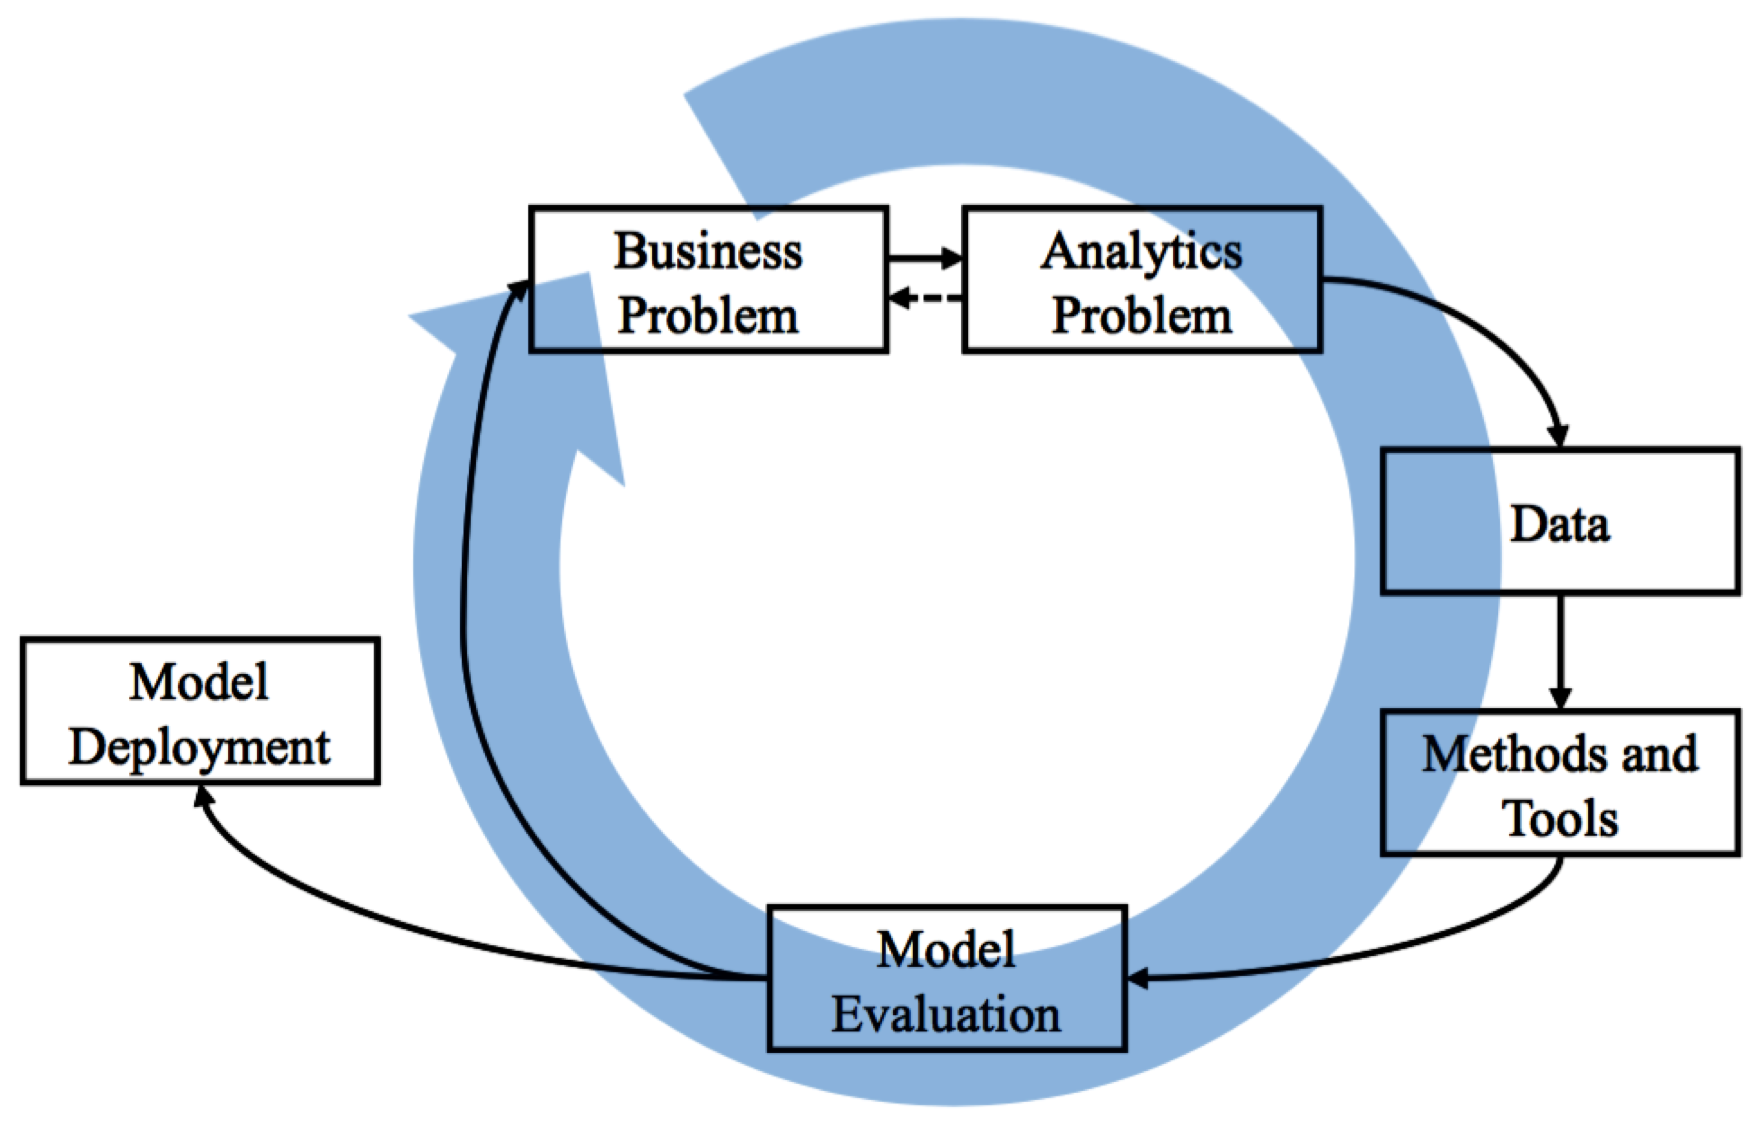
\includegraphics[width=1.05 \linewidth]{ModelLifecycle}
\label{fig:ModelLifecycle}
\caption{Model lifecycle.}
\end{figure}

\paragraph{Lifecycle governance}

A good lifecycle process:
\begin{itemize}
\item helps minimizing the cost and efforts for developing and maintaining the model.
\item \textit{allocates the users in a company clear roles.}
\item defines the roles of different departments involved.
\item defines the \textit{escalation processes} and \textit{decision making processes}.
\end{itemize}

\paragraph{Best practices}

\begin{itemize}
\item Do the documentation during the project (since things get forgotten quickly, there is no time for documenting after the project, people may leave the project early).
\item Define the measure for model quality in advance in the context of the model.
\item Have the old data available in a form s.t. one can readily recompute the different measures.
\item Define the frequency with which the model should be evaluated.
\item Do not only train users but also re-assess how they are using the model and the results and if necessary train the users again.
\item Evaluate the business benefit on a regular basis as it can diminish.
\end{itemize}

\section{Soft skills}

A data analytics professional needs the ability to convince, or explain the problem, problem solution and implications. \\
Thus a data analytics professional needs the following:
\begin{itemize}
\item \emph{Communication skills:} the ability to communicate with a client/employer/stakeholder regarding the framing of a business and an analytics problem.
\begin{itemize}
\item find the deep underlying motives of any client engagement
\item question until it is clear what the problem is and how a solution can be attempted
\item do not come up with proposals or solutions too early
\end{itemize}
\item \emph{Background and position:} the understanding of the background of the client/employer/stakeholder regarding his/her organization and specific industry focus.
\begin{itemize}
\item an organizational chart can help but might be insufficient
\item observe the inter- and intra-office communication since it often reveils the ''pecking order'' or internal group dynamics
\item take note of the people in the project management meetings and about their presence and behaviours since these are indicators of their status within the organization \\
$\Rightarrow$ stakeholder matrix
\end{itemize}
\item \emph{Clarifying the analytics process:} the ability to explain the findings of a the analytics process in sufficient details to ensure clear understanding by the client/employer/stakeholder.
\begin{itemize}
\item the data analytics professional is at the heart of the whole process and thus needs to have a complete understanding
\item ensure that your questions and comments are seen as necessary to the process, not as intrusive and time wasting
\item thus, be transparent and explain in simple words why you need certain information
\item translate between technical jargon and acronyms
\end{itemize}
\end{itemize}

\paragraph{Stakeholder matrix}

\begin{itemize}
\item \textit{Roles and responsibilities:} \\
What is he/she in charge of or expected to manage?
\item \textit{Business objectives and metrics:} \\
What does he/she want to achieve? How does he/she measure success? How is he/she evaluated?
\item \textit{External challenges:} \\
What external factors or industry needs might make it more difficult to reach his/her objectives?
\item \textit{Strategies and initiatives:} \\
What likely strategies and initiatives are in place to help achieve his/her objectives?
\item \textit{Internal issues:} \\
What likely issues does the organisation face that could prevent/hinder goal achievement?
\item \textit{Primary interfaces:} \\
Who are peers, subordinates, superiors, and outsiders with whom he/she frequently interacts?
\item \textit{Status quo:} \\
What is his/her status quo relevant to the project?
\item \textit{Change drivers:} \\
What would cause him/her to change from what is currently being done?
\item \textit{Change inhibitors:} \\
What would cause him/her to stay with the status quo, even if they are not happy with it?
\end{itemize}

\begin{figure}[H]
\centering
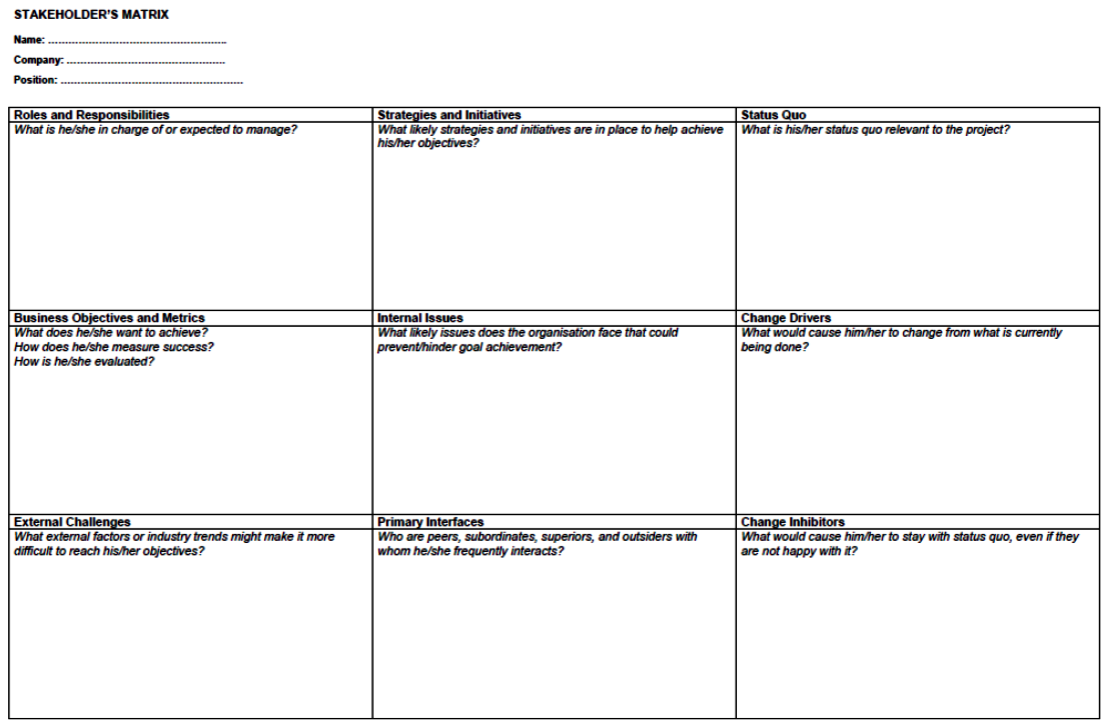
\includegraphics[width=1.05 \linewidth]{StakeholderMatrix}
\label{fig:StakeholderMatrix}
\caption{Structure of a stakeholder matrix.}
\end{figure}

\section{Excurses}

\subsection{Sentimental analysis}

\paragraph{Introduction}

\begin{itemize}
\item \emph{user-generated content:} reviews of products, blogs, forums, groups (all in the internet)
\item Nowadays, instead of conducting surveys, one simply has to mine the corresponding weg pages and extract the relevant information IOT get to know about the public opinion of a product or company.
\item \textit{Difficulties to find this information:} huge volume of data, unstructured data, data might be hidden in a certain blog, text and opinions are not straight-forward (e.g. irony, reversing expressions)
\end{itemize}

\paragraph{Definitions}

\begin{itemize}
\item \emph{Sentiment or opinion analysis:} extracting subjective information out of data by the use of natural language processing or text mining.
\item \emph{Natural language processing:} analyzing, understanding, generating and interacting with the language that humans use for interactions with computers in both written and spoken contexts using natural human languages instead of computer languages; area of computer science and artificial intelligence.
\item \emph{Text mining:} analyzing text and gathering information out of it by using pattern analysis techniques.
\item \emph{Object ($o$):} an entity which can be a product, person, event, organization or topic. \\
The object $o$ is associated with a pair: $o: (T,A)$, where $T$ is a hierarchy of components (or parts), sub-components, etc. and $A$ is a set of attributes (properties) of $o$. \\
Each component has its own set of sub-components and attributes.
\item \emph{Opinionated document ($d$)}: a product review, a forum post or a blog that evaluates a set of objects. \\
In the most general sense, $d$ consists of a sequence of sentences $d=\lbrace s_1,s_2,\ldots,s_m \rbrace$.
\item An \emph{opinion passage} on a feature ($f$) of an object $o$ evaluated in $d$ is a group of consecutive sentences in $d$ that expresses a positive or negative opinion on $f$.
\item \emph{Explicit feature:} $f$ is called an explicit feature in $s$ if $f$ or any of its synonyms appears in a sentence $s$.
\item \emph{Implicit feature:} if neither $f$ nor any of its synonyms appear in $s$ but $f$ is implied.
\item \emph{Opinion holder ($h$):} the person or organization that expresses the opinion.
\item An \emph{opinion} on a feature $f$ is a positive or negative view, attitude, emotion or appraisal on $f$ from an opinion holder.
\item The \emph{opinion orientation ($oo$)} on a feature $f$ indicates whether the opinion is positive, negative or neutral.
\item \emph{Model of an object:} an object $o$ is represented with a finite set of features, $F = \lbrace f_1,f_2,\ldots,f_n \rbrace$, which includes the object itself as a special feature. \\
Each feature $f_i \in F$ can be expressed with any one of a finite set of words or phrases $W_i = \lbrace w_{i1},w_{i2},\ldots,w_{im} \rbrace$, which are synonyms of the feature, or indicated by any one of a finite set of feature indicators $I_i = \lbrace i_{i1},i_{i2},\ldots,i_{iq} \rbrace$ of the feaute.
\end{itemize}

\paragraph{Model of an opinionated document}

\begin{itemize}
\item A general opinionated document $d$ contains opinions on a set of objects $\lbrace o_1,o_2,\ldots,o_q \rbrace$ from a set of opinion holders $h_1,h_2,\ldots,h_p$. \\
The opinions on each object $o_j$ are expressed on a subset $f_j$ of features of $o_j$. \\
An opinion can either be direct or comparative.
\item \emph{Direct opinion:} a quintuple $(o_j, f_{jk}, oo_{ijkl},h_i,t_l)$ \\
For feature $f_{jk}$ that opinion holder $h_j$ comments on, he/she chooses a word or phrase from either the corresponding synonym set $W_{jk}$, or a word or phrase from the feature indicator set $I_{jk}$ to describe the feature.
\item \emph{Comparative opinion:} expresses a relation of similarities or differences between two or more objects, and/or object preferences of the opinion holder based on some of the shared features of the objects. \\
Usually the \emph{comparative or superlative form} of an adjective or adverb is used.
\end{itemize}

\paragraph{Objective of mining direct opinions:}

Given an opinionated document $d$,
\begin{enumerate}
\item Discover all opinion quintuples $(o_j, f_{jk}, oo_{ijkl},h_i,t_l)$ in $d$.
\item Identify all synonyms ($W_{jk}$) and feature indicators ($I_{jk}$) of each feature $f_{jk}$ in $d$.
\end{enumerate}

\paragraph{Erroneous sentimental analysis}

E.g. denials and irony might be interpreted erroneously.

\subsection{European Statistic Code of Practice}

\begin{itemize}
\item \emph{Vision:} becoming a world leader in statistical information services; programme of harmonized European statistics as basis for democratic processes and progress in society
\item \emph{Mission:} provide the EU, the world and the public with independent high quality information on the economy and society on all levels and make information available to everyone for decision-making purposes, reasearch and debate
\end{itemize}

\paragraph{Code of Practice}

\begin{itemize}
\item \emph{Institutional environment}
\begin{itemize}
\item Professional independence
\item Mandate for data collection
\item Adequacy of resources
\item Commitment to quality
\item Statistical confidentiality
\item Impartiality and objectivity
\end{itemize}
\item \emph{Statistical processes}
\begin{itemize}
\item Sound methodology
\item Appropriate statistical procedures
\item Non-excessive burden on respondents
\item Cost effectiveness
\end{itemize}
\item \emph{Statistical output}
\begin{itemize}
\item Relevance
\item Accuracy and reliability
\item Timeliness and punctuality
\item Coherence and comparability
\item Accessibility and clarity
\end{itemize}
\end{itemize}

\subsection{System dynamics}

\paragraph{Definition}

\begin{itemize}
\item System Dynamics (SD) is a methodology for framing, modelling and understanding the dynamcis of a complex system.
\item It used for the understanding of non-linear behaviour of systems and to support system thinking.
\item SD is suitable for systems that:
\begin{itemize}
\item are dynamic and evolving over time.
\item are non-linear.
\item have accumulations and delays.
\item have feedback loops.
\end{itemize}
\end{itemize}

\paragraph{Patterns of behaviour}

\begin{itemize}
\item Typical variables are: \\
cost, sales, revenue, profit, market share, risk, etc.
\item Typical patterns of behaviour over time are: \\
exponential, goal-seeking, S-shape, oscillation
\item Often one of the first three patterns is combined with oscillation whose amplitude gradually declines over time.
\end{itemize}

\paragraph{Loops}

\begin{itemize}
\item \emph{Feedback loop} or \emph{causual loop:} a closed sequence of causes and effects, i.e. a closed path path of action and information (thus each element part of this subsystem influences itself)
\begin{itemize}
\item \emph{Self-reinforcing (R):} positive feedback
\item \emph{Self-correcting/balancing (B):} negative feedback \\
Remark: a balancing loop has always a goal/natural level
\end{itemize}
\item \emph{Open loop:} a linear chain of causes and effects which does not close back on itself
\end{itemize}

\paragraph{Loop diagrams}

\begin{itemize}
\item \emph{Elements:} variables, describe as nouns
\item \emph{Actions:} represented by arrows
\item Ensure the definition makes it clear which direction is up or down, i.e. prefer the \textit{positive sense in naming} a variable/action.
\item Causual links should imply a direction of causation, but not simply a time sequence.
\item Think about possible \textit{unexpected side effects}.
\item Negative feedback loops always have \emph{a goal}.
\item Include elements for both the \emph{actual value} of an element and the \emph{perceived value}.
\item Distinguish between \emph{short-term} and \emph{long-term consequences} with different loops.
\item If a link requires some explanation, then add intermediate elements inbetween.
\item Keep the diagramm as simple as possible.
\end{itemize}

\begin{figure}[H]
\centering
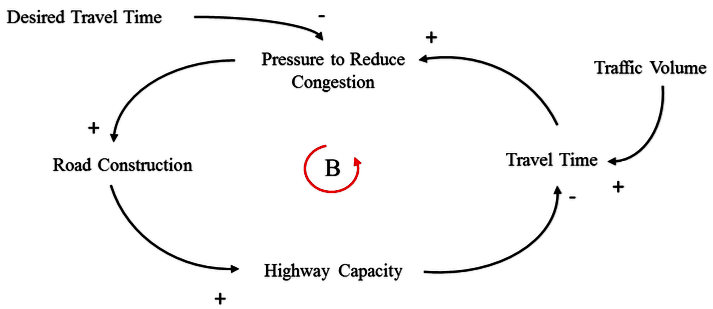
\includegraphics[width=1.05 \linewidth]{LoopDiagram}
\label{fig:LoopDiagram}
\caption{Loop diagram for the relationship between highway capacity and road congestion.}
\end{figure}

\paragraph{Stock and flow diagrams}

\begin{itemize}
\item Consider \emph{stocks}, \emph{in-} and \emph{outflows}, and \emph{auxiliary variables}.
\item Every stock and flow diagramm has \textit{at least one source}, \textit{one sink} (i.e. stocks outside the model) and \textit{one stock}.
\item Usually every stock has at least one in- and one outflow, each regulated by a valve.
\item \textit{Translation of elements from the loop diagram to the stock and flow diagram:}
\begin{itemize}
\item \emph{Stock:} an inventory which contains items where the amount of items can decrease or increase
\item \emph{Valve:} a variable regulating the in- or outflow of a stock, might be itself regulated by a stock or an auxiliary variable
\item \emph{Auxiliary variable:} elements that depict a certain dynamics but are neither stocks nor valves
\end{itemize}
\item \emph{Feedback loops:}
\begin{itemize}
\item Valves that regulate stocks but which are in return also regulated by stocks may replicate feedback loops from the loop diagram.
\item Such feedback loops may also incorporate auxiliary variables (i.e. elements of causual loop diagrams that are neither stocks nor valves).
\item Usually, every stock direcly or indirectly (via an auxiliary variable) reinforces its outflow valve. \\
\textit{The logic behind:} since the valves depict rates but not ratios and assuming that the outflow ratios remain constant, it follows that if a stock increases also its outflow rate (i.e. decrease of elements per time unit) increases. \\
Thus, each stock/outflow valve subsystem usually generates a balancing feedback loop (but which might be incorporated into a larger reinforcing loop).
\end{itemize}
\end{itemize}

\begin{figure}[H]
\centering
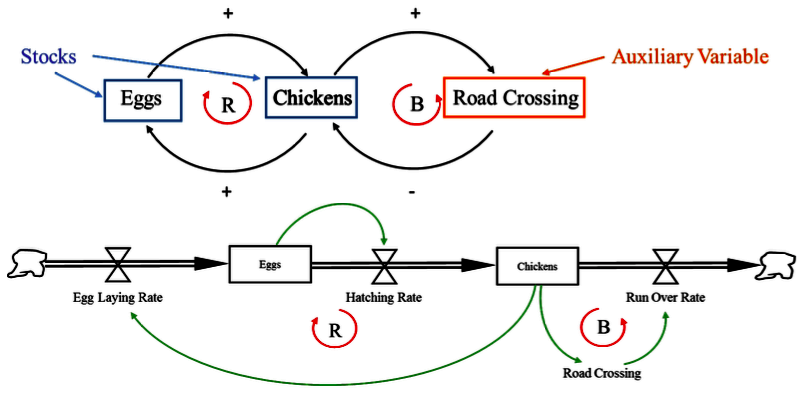
\includegraphics[width=1.05 \linewidth]{StockFlowDiagram}
\label{fig:StockFlowDiagram}
\caption{Loop diagram translated into a stock and flow diagram of a chicken and egg dummy system.}
\end{figure}

\columnbreak
\begin{center}
\textit{intentionally left blank}
\end{center}
\vfill

\section*{Abbreviations}

\begin{description}[style=multiline,leftmargin=1cm,font=\textbf]
%\item[a.s.] almost surely
%\item[BM] Brownian motion
\item[IOT] in order to
%\item[PDE] partical differential equation
\item[RV] random variable
%\item[SDE] stochastic differential equation
\item[s.t.] such that
\item[w.r.t.] with respect to
\end{description}

\section*{Disclaimer}

\begin{itemize}
\item This summary is work in progress, i.e. neither completeness nor correctness of the content are guaranteed by the author.
\item This summary may be extended or modified at the discretion of the readers.
\item Source: Lecture Data Analytics in Organisations and Business, autumn semester 2015/16, ETHZ (lecture slides, script and exercises). Copyright of the content is with the lecturer.
\item The layout of this summary is mainly based on the summaries of several courses of the BSc ETH ME from Jonas LIECHTI.
\end{itemize}

\end{multicols*}

\end{document}